\documentclass[11pt]{book}
\usepackage[usenames,dvipsnames]{color}
\usepackage{array}           % For double-column exercises.
\usepackage{longtable}       % For double-column exercises.
\usepackage[normalem]{ulem}  % For strikethrough.
\usepackage{paralist}
\usepackage{enumitem}        % To "resume" enumerated lists.
\usepackage{epsfig}
\usepackage{afterpage}
\usepackage{multicol}
\usepackage{fancybox}
\usepackage{makeidx}
\usepackage{textcomp}
\usepackage{fancyvrb}
\usepackage{footnote}
\usepackage{makecell}
\usepackage{amsmath,amsthm,amsfonts,amssymb,latexsym}
\usepackage{MnSymbol}
\usepackage{wasysym}
\usepackage[width=.9\textwidth,singlelinecheck=true,skip=1pt,font=small,labelfont=bf]{caption}
\newcommand{\freakingtilde}{\raisebox{0.5ex}{\texttildelow}}
\makesavenoteenv{tabular}  % to allow footnotes in tables
%\captionsetup{width=.9\textwidth}

%\usepackage{enumerate}

\makeindex

\newenvironment{custommargins}[2]%
  {\addtolength{\leftskip}{#1}\addtolength{\rightskip}{#2}}{\par}

% Set left margin - The default is 1 inch, so the following
% command sets a 2-inch left margin.
\setlength{\oddsidemargin}{1in}
\setlength{\evensidemargin}{0in}
% Set width of the text - What is left will be the right margin.
% In this case, right margin is 8.5in - 1.25in - 6in = 1.25in.
\setlength{\textwidth}{5.5in}

% Set top margin - The default is 1 inch, so the following
% command sets a 0.75-inch top margin.
\setlength{\topmargin}{.75in}

% Set height of the text - What is left will be the bottom margin.
% In this case, bottom margin is 11in - 0.75in - 9.5in = 0.75in
\setlength{\textheight}{7.25in}

\setlength{\parindent}{0pt}
\setlength{\baselineskip}{1.5pt}
\setlength{\parskip}{6pt}

\begin{document}

\title{Blueprints: Creating, Describing, and Implementing\\Designs for Larger-scale Software
Projects\\{\small version 1.0.0}}
\author{Stephen Davies, Ph.D.\\Computer Science Department\\University of Mary Washington}
\date{}
\maketitle

\frontmatter

\renewcommand{\contentsname}{Contents at a glance}

\setcounter{tocdepth}{0}
\tableofcontents

% 
\chapter{Preface}
Coming soon.


\setcounter{chapter}{0}

\mainmatter

\chapter{Getting off the ground}
\label{ch:gettingOff}

\index{command line}
\index{Linux}
\index{Unix}
Before we begin our study of object-oriented systems proper, we'll introduce
the command-line toolset we'll be using to construct our programs. We'll take
each of the most important tools out of our toolbox, lay them out before us on
a little mat, and learn what they're for.

\section{Why the command line?}

\index{CLI (command-line interface)}
\index{GUI (graphical user interface)}
Developing software in a command-line environment (sometimes abbreviated
``CLI'' for \textbf{command-line interface}, as opposed to a
``GUI\footnote{Commonly pronounced ``gooey.''}'' or \textbf{graphical user
interface}) involves typing white text in little black boxes. It requires
memorizing and regurgitating a variety of obscure commands. It demands exact
adherence to an inconsistent syntax, and exacts heavy penalties for mistakes,
all while providing only a very crude and clunky-looking interface.

It's natural to wonder why we would want to do this. After all, aren't
computer systems immeasurably more sophisticated now? If even end users run
fancy, graphical, forgiving apps, shouldn't computer scientists expect even
easier-to-use and sexier-looking stuff?

It may seem so, and in terms of the \textit{power} the tools provide, we'll
discover that indeed software developers are aptly equipped. But in some ways
it's a false expectation to assume that our toolset would be as \textit{easy}
to operate as that of an everyday user. After all, which is easier: to drive a
car, or to be a mechanic? Even though I enjoy cruise control and
auto-adjusting seats, I don't find it strange at all to learn that mechanics
still use socket wrenches to adjust piston assemblies.

Much of what makes a CLI so powerful is its expressiveness. A driver can press
any of the three or four cruise control functions the manufacturer provided.
But a mechanic can take any of hundreds of tools, tweak dozens of different
parts, and combine these adjustments in uncountable ways. That's the kind of 
flexibility the command line provides.

The difference between a CLI and a GUI is that with the latter, the user can
essentially do \textit{only what the tool designer anticipated she would want
to do.} There's no way she can express something that isn't one of the
tailor-made menu options.

When you use the command line, think of it as composing sentences, word by
word. A GUI comes with a repertoire of standard sentences you can choose from.
That makes it easy to do standard things, and hard to make silly mistakes. But
a CLI, being inherently language-based, is immeasurably more flexible. You can
write any (legal, grammatically correct) sentence you choose, even one the
designers of the CLI never thought of, and even one that you didn't know you'd
want to type until a moment ago. The bits and pieces can be combined in a
myriad of ways, just as nouns and verbs can.

\index{Finlayson, Ian}
There are other reasons as well that many developers live on the command line.
Among them are\footnote{Thanks to Ian Finlayson for capturing much of this
list.}:

\begin{itemize}
\itemsep.1em

\item \textbf{Speed.} It turns out to be way, way faster to type commands --
in combination with the various shortcuts and recall/edit operations -- than
it is to sift through menu options and such with a mouse. Trust me.

\index{remote access}
\index{shell}
\item \textbf{Remote access.} When you're running programs on your own device,
it's possible to do it with a GUI. But computer scientists very often have to
connect over the network to distant machines in order to tell them what to do.
Every time you need to configure a web server, for instance, or update a
publicly-accessible database, or run a time-consuming job on a parallel
cluster, or correct the data on your mobile device, you need a way to issue
commands to another machine through a very low-bandwidth channel. Opening a
command line ``shell'' to that remote device is by far the most common and
effective way to do this.

\index{scriptability}
\item \textbf{Scriptability.} There's just no good way to automate a sequence
of GUI operations. To explain to someone else how to accomplish something, you
have to painfully walk them through each operation (``go to the Start menu and
find Accessories, then in the Math menu choose Calculator...when it comes up,
right-click in the background and enable Advanced Options...'') which is
tedious and error-prone. It'd be nice if you could just send them a custom
command which would do all that. As a matter of fact, it would be nice if
\textit{you} could make a custom command which would do all that, so that you
could execute it many times without rehashing the same rigmarole. You'll find
that CLIs are eminently automatable in this way. You can create custom
commands called ``scripts'' that are combinations of other interacting
commands, and in this way you become master of your whole world.

\index{Cygwin}
\index{Mac OS X}
\index{Microsoft Windows}
\index{Raspberry Pi}
\index{Kindle}
\index{Terminal application}
\item \textbf{Consistency.} Graphical user interfaces are more different from
each other than CLIs are. Partly this is because nearly any CLI you're likely
to use is Unix/Linux-based\footnote{For our purposes, you can consider the
terms ``Unix'' and ``Linux'' exact synonyms. The Mac OS X command line
(available through the ``Terminal'' app) is Unix-based, too. Windows machines
aren't, but programs like ``Cygwin'' can be downloaded for free and provide a
Linux-like command-line veneer over the operating system.}, and hence they all
``speak the same language.'' It's great to be able to log on to different
laptops, web servers, your phone, your Kindle, or a Raspberry Pi and get the
same prompt that understands the same stuff.

\index{Linux}
\index{Unix}
\index{CLI (command-line interface)}
\item \textbf{Stability.} CLIs rarely change. When they do, it's very very
rarely in a non-backwards-compatible way. Every time a new graphical user
interface is released, you have to go through a period of hunting around and
finding out where everything is. With Unix/Linux, you can literally run
commands that were written last century and they will likely still work as is.

\end{itemize}

There's always a few students who despite the above benefits, resist learning
this material at first. I get it. It's like learning a new language, and the
immense effort to understand an alien world sure doesn't feel like it's going
to pay off any time soon. All I can say is that if you're not convinced it's
worth it, for now just think of it as something you have to master ``just
because your professor and the industry says so.'' My hope is that by the end
of this course, you're pleasantly surprised by seeing some payoff for your
hard work.


\section{The filesystem}
\index{filesystem}
\index{file}
\index{tree}
\index{directory}
\index{folder}

Okay. The backdrop for all our use of the Linux command-line interface is the
\textbf{filesystem}.\footnote{Often, not always, written as a single word as I
have it here.} Any general-purpose computer, no matter its architecture or OS,
has an area of permanent storage for user data. Interestingly, and
conveniently, they're all organized in pretty much the same way: as a
\textbf{tree} of \textbf{files} and \textbf{directories}. (Windows/Mac users
will be familiar with the term ``\textbf{folder},'' which \textit{means exactly
the same thing as ``directory.''}) In what follows, we'll be using a different
syntax (text instead of visual icons) to work with what is conceptually the
same organizational structure you're used to on your own computer.

\subsection{Files and directories}

\index{filesystem extension}
A file is simply any named chunk of stuff on your disk. Images, .mp3 tunes,
Word docs, and (importantly) plain text files are all in this category. On
Windows, you're used to each of these files having a filesystem ``extension''
designating its type: ``.doc'' means a Word doc, and ``.jpg'' means an image
file, for example. This is sort of true with Linux, although the rules are
a bit looser. Not all files have extensions at all, and when they do, it's
more a signal that they're intended to be treated a certain way than a
hard-and-fast requirement.

\index{java file@\texttt{.java} file}
The most important files you'll work with in this class will have a
\texttt{.java} extension. These are your Java source files. You'll also work
with other various supporting files to make all the tools work correctly.
It's important to realize that \textit{a file is fundamentally just some data,
which can theoretically be opened and dealt with by any program}. When we say
that HamletPaper.doc ``\textit{is}'' a Word doc, what we really mean is that
its data is formatted in a certain way that the Microsoft Word application
expects to see, so it can render it on the screen for editing. But it is
possible to open that same HamletPaper.doc file with other programs and
manipulate its contents. This may seem sketchy, but it is actually a force for
good.

In particular, you'll be tempted this semester to think of a \texttt{.java}
file as ``a \texttt{vim} file,'' in the same way that you may think of an
\texttt{.xls} file as ``an Excel file.'' I hope to eventually break you of this
habit, as you learn to see files as text or data that is actually independent
of what kind of program might be used to open and manipulate it.

\index{directory}
A directory is a container for files \textit{and also other directories}. That
last italicized phrase is what gives rise to the overall tree structure of the
filesystem, as discussed in the following section.

\index{Foreman, George}
By the way, every file and directory \textit{in a particular directory} must
have a unique name. You can't have a file called ``DireStraits.mp3'' and
another one also called ``DireStraits.mp3'' sitting there in the same folder:
it's a name collision. However, it's perfectly permissible to have two files
with the same name in different directories. This is kind of like how there
isn't more than one ``Stephen'' in my immediate family (that would be
confusing\footnote{With apologies to boxing legend George Foreman, who named
all four of his children ``George.'' That practice is not
filesystem-compatible.}), but there are of course many ``Stephens'' in the
world.

\subsection{The filesystem tree}

\index{tree}
\index{filesystem}
\index{directory!parent}
\index{parent directory}
The files and directories in a filesystem form a nested, hierarchical
structure called a \textbf{tree} (see Fig.~\ref{fig:tree}). I have drawn two
kinds of nodes in this tree: directories (yellow ovals) and files (blue
boxes). As expected, some of the directories have arrows coming out of them,
but none of the files do. The elements that a directory is pointing to are the
contents it contains: \textit{e.g.}, the left-most ``\texttt{america}''
directory contains another directory (``\texttt{nation}'') and also the file
\texttt{A.txt}. We use the term \textbf{parent directory} to mean the
directory immediately above an entry in the filesystem; the left-most
\texttt{A.txt} file's parent directory is the \texttt{america} directory we
just spoke of.

\begin{figure}[ht]
\centering
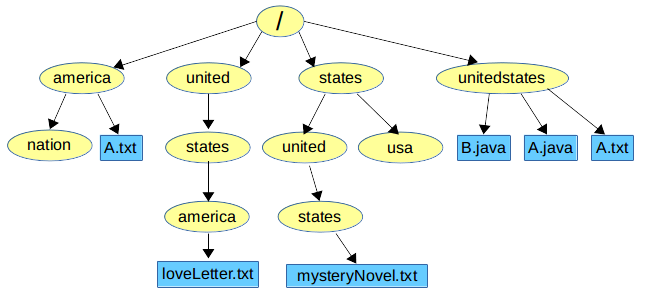
\includegraphics[width=0.9\textwidth]{tree.png}  %650x300
\caption{The Linux filesystem, in pictorial form.}
\label{fig:tree}
\end{figure}

Note that in order to keep you on your toes, I've given several entries in
this example filesystem the same name: in addition to a couple different
\texttt{america}s, we've got several \texttt{states}, multiple different
\texttt{A.txt}s, etc. In no case, however, are the duplicately-named entries
in the same directory. (Convince yourself of that fact.)

\subsubsection{Only one surprise}

\index{Microsoft Windows}
So far this is pretty easy. And it won't get much harder. But here's the one
thing you have to get used to: with a CLI, \textit{we won't ever actually see
that filesystem picture visually.} It's there, but we don't explicitly view it
in graphical form. Instead, there will be a textual way of referring to every
file and directory. It's straightforward, but can be a bit of a shock to those
coming from point-and-click systems like Windows.

\subsection{The ``current'' (or ``working'') directory}

\index{directory!current}
\index{directory!working}
\index{current directory}
\index{working directory}
One vital concept to grasp is that every time we issue a command or run a
program in Linux, we are doing so \textit{within the context of a particular
directory}. Conceptually, we think of being ``in'' a certain directory at any
point in time. We call this directory ``the \textbf{current directory}'' or
``the \textbf{working directory}'', and we'll learn commands to find out what
it is and to change it to something else.

Which one we're ``in'' has a crucial impact on what happens when we execute a
command. For instance, if our current directory is the far-left
\texttt{america} directory, and we issue a command that does something to
``\texttt{A.txt}'', it would act on the left-most \texttt{A.txt} file, since
it's the one within the current directory. But if our current directory were
\texttt{unitedstates}, ``\texttt{A.txt}'' would instead mean the far-right blue
node.

I've found that failure to understand the current directory is one of the most
common trouble spots for beginning Linux programmers.

\subsubsection{The root directory}

\index{directory!root}
\index{root directory}
\index{tree}
Okay, back to the filesystem as a whole. At the top of the tree is the
\textbf{root directory}, which has no parents. (This is often disorienting to
non-computer-scientists, since in the real world trees actually grow
\textit{up}, not down. But in computer science, we always draw trees growing
down from the root.)

\index{backslash}
\index{forward slash}
\index{slash}
\index{Microsoft Windows}
The root directory is the anchor point of the entire filesystem: it ultimately
contains everything under it. It also has a very strange name: ``\texttt{/}'',
pronounced ``slash.'' (This is a ``forward slash,'' by the way, to the left of
your right-most Shift key, not a ``backslash.'' Oddly, most Windows systems
use a backslash ``\texttt{\textbackslash}'' for this instead.) Stay awake,
because this ``\texttt{/}'' character will shortly mean something very
different as well.

\subsubsection{Paths}

\index{path}
\index{directory}
\index{file}
It should be apparent to you that as a consequence of this nested tree
structure, you can ``reach'' every element from the root directory by
traversing from arrow to arrow. Furthermore, you can do so in only one way.
For instance, the \texttt{B.java} file can be reached from the root by going
from ``\texttt{/}'' to \texttt{unitedstates} to \texttt{B.java}. And that's the
\textit{only} way to get there. You can reach \texttt{loveLetter.txt} by going
from ``\texttt{/}'' through \texttt{united}, \texttt{states}, and
\texttt{america}, in that order. This is true for every file and directory.

What this means is that every entry has a unique \textbf{path}, and we can
express it in text as well as in a diagram. Take the \texttt{B.java} file for
example. Its path is:

\quad\quad \texttt{/unitedstates/B.java}

\index{slash}
Look very carefully at that string as we dissect it. The most important thing
to grasp is that the two slash (``\texttt{/}'') characters \textit{each mean
something different}. The first one means ``the root directory, which is
called slash.'' But the second one is merely a separator, delimiting the
\texttt{unitedstates} from the \texttt{B.java}. So this path means
``\textit{start at the root directory}, go down to its \texttt{unitedstates}
entry (which is a directory), and there you have the \texttt{B.java} file.''

Similarly, the path to \texttt{loveLetter.txt} is:

\quad\quad \texttt{/united/states/america/loveLetter.txt}

\index{slash}
(Note that the slash between \texttt{united} and \texttt{states} makes all the
difference in the world: if it weren't there, we'd be starting our descent
through the right-most \texttt{unitedstates} directory as before.)

\index{path!absolute}
\index{absolute path}
\index{planet}
\index{path!relative}
\index{relative path}
These paths are called \textbf{absolute paths} because they \textit{start with
a slash}. This means that they give the complete, start-from-the-top position
of a particular file or directory. It's kind of like referring to a building
by its complete address, including city, state, zip code, country, and planet.
Often we want a short-hand way of referring to an entry without specifying its
entire absolute path. To do so, we use a \textbf{relative path}.

\index{directory!current}
\index{current directory}
A relative path is relative \textit{to the current directory}. And it does
\textit{\textbf{not}} begin with a slash. Instead, it gives directory names,
separated by slashes, indicating where to start descending \textit{from the
current directory}.

For example, let's say the current directory was ``\texttt{/states}''. And
suppose I used this relative path:

\quad\quad \texttt{united/states/mysteryNovel.txt}

(Note \textit{carefully} that it has \textit{no} initial slash!) This relative
path would instruct us to \textit{start at the current directory}
(\texttt{/states}) and from there traverse down to \texttt{united},
\texttt{states}, and then finally \texttt{mysteryNovel.txt}. Obviously, where
you end up is critically dependent on where you start -- on what the current
directory is.

\index{directory!current}
\index{current directory}
To test your understanding, realize that in this case where the current
directory is \texttt{/states}, there is no such file called
\texttt{united/states/america/loveLetter.txt}. In fact, even 
\texttt{united/states/america} doesn't exist. However, if we changed the
current directory to be the root (``\texttt{/}''), suddenly the relative path
\texttt{united/states/ america/loveLetter.txt} would be legit.

\section{Linux A-B-C's}

\index{Unix}
\index{Linux}
\index{filesystem}
\index{file}
\index{directory}
With the filesystem always hovering in the background, let's introduce the
first basic Linux commands to work with the files and directories. These
commands are so basic that they're like the alphabet of speaking any Linux
sentence. Using them should eventually be as familiar and effortless as
clicking the mouse.

\index{prompt}
\index{dollar sign (\texttt{\$})}
In all that follows, I will precede anything you are to type on the Linux
command line with a dollar sign \textbf{prompt}:

\begin{Verbatim}[fontsize=\small]
$
\end{Verbatim}

To execute a command, you do \textit{not} type the prompt itself: it's just
there to indicate ``now is an appropriate time and place to enter a Linux
command.'' Just type the stuff after it.

\index{directory!current}
\index{current directory}
Also, depending on your system and configuration, your prompt may look
different or have other information in it. One common setting, for instance,
is for the current directory to always appear as the prompt. (I personally
hate that, since it makes some commands start at different horizontal
locations as I work, plus it consumes a lot of space.) No matter what, though,
just mentally substitute ``the dollar sign'' for ``whatever your Linux prompt
is.''

\newcommand{\bigline}{\begin{center} \line(1,0){300} \end{center}}


\begin{enumerate}
\itemsep.1em
\item \textbf{\texttt{pwd}}

\index{pwd@\texttt{pwd}}
Your first command stands for ``\textbf{p}rint \textbf{w}orking
\textbf{d}irectory,'' and simply tells you what the current directory is at any
point in time. For example:

\begin{Verbatim}[fontsize=\small]
$ pwd
/united/states
\end{Verbatim}

tells you that you're currently ``in'' the \texttt{states} directory, which is
contained within the \texttt{united} directory, which is contained within the
root directory.

\textbf{Tip:} get in the habit of typing \texttt{pwd} a \textit{lot},
especially at first. Get ingrained in your brain the concept of ``where am I
in the filesystem right now?'' because it matters, yet is not in your face
except when you type this command.

\bigline
\item \textbf{\texttt{cd}}

\index{cd@\texttt{cd}}
\texttt{cd} stands for ``\textbf{c}hange \textbf{d}irectory'' and is how you
move to another place. You give it an \textbf{argument} (kind of like passing
a parameter to a function call in a programming language, although we don't
use parentheses or commas here) which is where you want to go:

\begin{Verbatim}[fontsize=\small]
$ cd  /america/nation
\end{Verbatim}

Here, I've specified an absolute path. If I now execute \texttt{pwd}, I see
that it worked:
\begin{Verbatim}[fontsize=\small]
$ pwd
/america/nation
\end{Verbatim}

\index{relative path}
\index{path!relative}
\index{absolute path}
\index{path!absolute}
More common is to specify a relative path. If we go back to our original
location:

\begin{Verbatim}[fontsize=\small]
$ cd  /united/states
$ pwd
/united/states
\end{Verbatim}

we can then say ``go \textit{from here} into the \texttt{america} directory'':

\begin{Verbatim}[fontsize=\small]
$ cd  america
$ pwd
/united/states/america
\end{Verbatim}

\index{cd@\texttt{cd}}
\index{pwd@\texttt{pwd}}
I can't overestimate how important it is to notice that in the previous
\texttt{cd} command, I did \textit{not} include a slash before
\texttt{america}. If I had, it would have been an absolute path, and I would
have gone to a completely different part of the filesystem:

\begin{Verbatim}[fontsize=\small]
$ cd  /america
$ pwd
/america
\end{Verbatim}

\subsubsection{``Special'' directory shortcuts}

\index{directory!shortcuts}
\index{special directory shortcuts}
This is a good time to mention that when you are specifying paths, there are
three very common shortcuts that you'll want to know about.


\begin{itemize}
\itemsep1em

\index{directory!current}
\index{current directory}
\item The current directory: \texttt{\textbf{.}}

A plain-ol' dot (period) is used to mean ``the current directory.'' There's no
obvious uses for this yet, but believe me, it comes up \textit{all} the time,
so just memorize it. A useless example for now:

\begin{Verbatim}[fontsize=\small]
$ pwd
/united/states
$ cd  ./america
$ pwd
/united/states/america
\end{Verbatim}

So ``\texttt{./america}'' is another way of saying ``\texttt{america}''. (Told
you this example was useless.)

\item The parent directory: \texttt{\textbf{..}}

\index{directory!parent}
\index{parent directory}
More immediately useful is the double-dot, which means ``the parent of the
current directory.'' If we're in \texttt{/united/states} and want to go to
\texttt{/united}, one way to do it is:

\begin{Verbatim}[fontsize=\small]
$ cd  ..
$ pwd
/united
\end{Verbatim}

We can also join this with additional relative path stuff to move around the
hierarchy in various ways:

\begin{Verbatim}[fontsize=\small]
$ pwd
/states/united
$ cd  ../usa
$ pwd
/states/usa
\end{Verbatim}

\index{directory!sibling}
\index{sibling directory}
\index{directory!child}
\index{child directory}
Here we went to a ``sibling'' directory by ``going up one, and then down to a
different child.''

\item The home directory: \texttt{\textbf{\freakingtilde}}

\index{directory!home}
\index{home directory}
A shortcut for ``the home directory'' (which means ``the current directory when
you first log in'') is a tilde. It's commonly used in conjunction with other
relative path stuff, like the last double-dot example, above.

Your home directory (which you can verify by just typing \texttt{pwd} when
you first log in) will probably be something like \texttt{/home/joeschmo}.
Suppose it is. Then, if you type:

\begin{Verbatim}[fontsize=\small]
$ pwd
/somewhere/else/in/the/filesystem
$ cd  ~/shortStories/scifi
$ pwd
/home/joeschmo/shortStories/scifi
\end{Verbatim}

you can go to any of your subdirectories.

\end{itemize}

\bigline
\item \textbf{\texttt{ls}}

\index{ls@\texttt{ls}}
While \texttt{pwd} tells you what the current directory is, \texttt{ls}
command (``\textbf{l}i\textbf{s}t'') gives you its contents. If I type it while
in the \texttt{/america} directory, for instance, it tells me:

\begin{Verbatim}[fontsize=\small]
$ ls
nation   A.txt
\end{Verbatim}

there are the two entries from Figure~\ref{fig:tree}.

\index{ls@\texttt{ls}}
A few gotchas to be aware of here. First, there's no way from that listing to
tell that \texttt{nation} is a directory whereas \texttt{A.txt} is a file. If
you want to see that, you need to add the ``\texttt{-l}'' (a minus sign
followed by the lower-case letter ``ell'') option:

\begin{Verbatim}[fontsize=\small]
$ ls  -l
-rw-r--r-- 1 kyloren   sithlords   17 Sep  5 16:21 A.txt
drwxr-xr-x 2 kyloren   sithlords 4096 Sep  5 16:21 nation
\end{Verbatim}

Lots of clutter here. The key points:

\begin{compactitem}[-]
\item The far-left character on each line is either a ``\texttt{-}'' or a
``\texttt{d}'', indicating file or directory.
\index{file!owner}
\item Files in Linux have ``owners,'' meaning specific users who created them
and have permissions to manage them. Both of these entries are evidently owned
by user \texttt{kyloren}.
\item The \texttt{17} and \texttt{4096} are file sizes (in bytes).
\item You can see the date and time each entry was last modified.
\end{compactitem}

\index{long file listing}
\index{option}
The ``\texttt{-l}'' stands for ``\textbf{l}ong file listing.'' Most Linux
commands have a bevy of different options you can specify when you execute
them, most often beginning with a minus sign.

Another important one for the \texttt{ls} command is ``\texttt{-a}'' which
stands for ``\textbf{a}ll files, please.'' If that sounds like a strange
option, that's because it is. It turns out that \texttt{ls} by default doesn't
show you all the files; in particular, \textit{it omits those whose names
start with a dot (.).} Why? There are reasons. The only time this will be
relevant to you soon is when you want to work with the \texttt{.bashrc} file,
as described later in this chapter. You'd have to type ``\texttt{ls -a}'' in
your home directory to actually see it in the listing.


\bigline
\vspace{.1in}
\index{cd@\texttt{cd}}
\index{pwd@\texttt{pwd}}
\index{ls@\texttt{ls}}
*The above three commands -- \texttt{pwd}, \texttt{cd}, and \texttt{ls}, go
together like Rey, Finn, and Poe. Get in the habit of using them literally
every minute you're working on the Linux command line.
\vspace{.1in}
\bigline

\item \textbf{\texttt{mkdir}}

\index{mkdir@\texttt{mkdir}}
To create a directory in the first place, use the \texttt{mkdir} command and
give it the name:

\begin{Verbatim}[fontsize=\small]
$ mkdir  evilplans
\end{Verbatim}

This new \texttt{evilplans} directory will be created inside the current
directory.

Note carefully that \textit{making a directory does not automatically put you
in it!} Lots of beginners mistakenly think this will happen, but you can see
that it does not:

\begin{Verbatim}[fontsize=\small]
$ pwd
/home/kyloren
$ mkdir  evilplans
$ pwd
/home/kyloren
\end{Verbatim}

\index{cd@\texttt{cd}}
You have to \texttt{cd} as a separate step if you want to now be in
\texttt{evilplans}:

\begin{Verbatim}[fontsize=\small]
$ cd  evilplans
$ pwd
/home/kyloren/evilplans
\end{Verbatim}

\index{directory!parent}
A useful option to \texttt{mkdir} is the ``\texttt{-p}'' option which means
``make all \textbf{p}arent directories as necessary.'' This lets us create a
deeply-nested structure all in one fell swoop:

\begin{Verbatim}[fontsize=\small]
$ mkdir  -p  find/luke/skywalker/now
$ cd  find/luke/skywalker/now
$ pwd
/home/kyloren/find/luke/skywalker/now
\end{Verbatim}

\bigline

\item \textbf{\texttt{cp}}
\index{cp@\texttt{cp}}
\index{file!copying}

To make a copy of a file, use \texttt{cp} and give it \textit{two} arguments,
a source and a destination. If I type:

\begin{Verbatim}[fontsize=\small]
$ cp  A.txt  Q.txt
\end{Verbatim}

I will now have two exact copies of the file which can be independently
modified:

\begin{Verbatim}[fontsize=\small]
$ ls
nation   A.txt   Q.txt
\end{Verbatim}

I can also use this to make a (same-named) copy of a file to a different
location, by providing a directory as the second argument:

\begin{Verbatim}[fontsize=\small]
$ cp  A.txt  /states/usa
$ cd  /states/usa
$ ls
A.txt
\end{Verbatim}

\bigline

\item \textbf{\texttt{mv}}
\index{mv@\texttt{mv}}
\index{file!renaming}

\texttt{mv} has pretty much the same effect as \texttt{cp}, except that it
does not retain the original copy. This command can be used to rename a file
(``\texttt{\$ mv oldfilename newfilename}'') as well as to change a file's
location.

\bigline

\item \textbf{\texttt{vim}} (and \texttt{vimtutor})
\index{vim@\texttt{vim}}

It's really ludicrous to include this command in amongst all the others, when
its ins-and-outs could (and do) occupy entire textbooks in their own right.
\texttt{vim} is a text editor program with a zillion amazing features which
you will use this semester to write your programs. The normal way of creating
a file, in fact, will be this:

\begin{Verbatim}[fontsize=\small]
$ vim  notesOnTheResistance.txt
\end{Verbatim}

or this:

\begin{Verbatim}[fontsize=\small]
$ vim  DestroyGalacticRepublic.java
\end{Verbatim}

after which you will do loooooooooooots of other stuff way beyond the scope of
this book. That stuff will be cryptic and agonizing at first, but will
eventually become second-nature and give you the tremendous text editing power
you need to be a truly efficient software developer. It's kind of like
learning to use the Force for the first time.

\index{vimtutor@\texttt{vimtutor}}
For now, I'll make this (strong) suggestion: when you're first learning vim,
type this command (all one word) at the command line,

\begin{Verbatim}[fontsize=\small]
$ vimtutor
\end{Verbatim}

\index{Coke}
grab a Coke, and spend 30-40 minutes patiently reading and following the
instructions. This tutorial is quite good, and will teach you the very basics
of getting a file created and edited with this incredible tool.

\bigline

\item \textbf{\texttt{git}}
\label{introduceGit}
\index{git@\texttt{git}}
\index{version control system}

\texttt{git} is another one that doesn't really fit in this list, since it's
much more than just ``a command.'' For now, though, all you need to understand
is that it's a \textbf{version control system} that allows you to track and
manage the changes you make to your software over time. Up until now, you've
been dealing with the paradigm of ``the IDE always has the most recent copy of
my code, and that's the only version of it that exists.'' It turns out that
you'll need much more flexibility than that when you work on large systems.

Here's all you need to know at present:

\begin{compactitem}
\index{git@\texttt{git}!\texttt{git init}}
\index{repository@``repo'' (repository)}
\item The command ``\texttt{\$ git init .}'' (don't forget the dot at the end,
after a space) creates a git \textbf{repository}
(or ``\textbf{repo}'') in the current directory. That just means that your
current directory, and everything under it, are now ``under git's
management.'')
\index{git@\texttt{git}!\texttt{git add}}
\item You use ``\texttt{git add}'' to make git aware of
one or more files that you want it to track from that point forward. You'll
type ``\texttt{\$ git add }file1 file2 file3'' or however many files you want
to add at that point. Ordinarily you'll want to \texttt{git add} all of your
\texttt{.java} files.
\index{git@\texttt{git}!\texttt{git commit}}
\index{commit}
\index{snapshot}
\item When you've made a
significant change to one or more of your files that you want git to be aware
of, you'll enter this command:
\begin{Verbatim}[fontsize=\small]
$ git  commit  -a  -m  "A message describing the change."
\end{Verbatim}
Each such change is called a \textbf{commit}. Think of it as taking a
snapshot of your code that you can return to later.
\index{git@\texttt{git}!\texttt{git status}}
\index{git@\texttt{git}!\texttt{git log}}
\item ``\texttt{\$ git status}'' and ``\texttt{\$ git log}'' are two useful
commands that show the current state of your files as git sees them, and a
history of all the different commits you've made. Type them occasionally just
to get a feel for what kind of information they show.
\end{compactitem}

We'll talk much more about \texttt{git} later. For now, just know that it
exists, and type the commands verbatim when prompted.

\bigline
\item \textbf{\texttt{javac}} and \textbf{\texttt{java}}

\index{javac@\texttt{javac}}
\index{java@\texttt{java}}
\index{compiler}
\index{virtual machine}
\index{JVM (Java Virtual Machine)}
\index{JDK (Java Development Kit)}
\index{J2SE (``Java 2 Standard Edition'')}
\index{JRE (Java Runtime Environment)}

Now, finally to some programming stuff. On your Linux system, the Java
\textbf{compiler} (\textit{i.e.}, the program that converts your source code
into the form the computer needs to run it) is called \texttt{javac}, and the
\textbf{virtual machine} (the interpreter that runs your compiled code) is
called \texttt{java}. Both of these are part of the \textbf{JDK}, or ``Java
Development Kit,'' that you install in order to program in Java.\footnote{Just
to confuse you, the JDK has sometimes been called the ``Java SDK'' (``Java
Software Development Kit'') and the ``J2SE'' (``Java 2 Standard Edition'') in
the past, and you'll likely run across those acronyms as well. To confuse you
even more, the software you need to simply \textit{run} a Java program (as
opposed to writing your own) is called the ``JRE'' -- Java Runtime
Environment. Finally, to confuse you yet further, Java version numbers were
originally all ``one-dot-something'' (like ``Java 1.3'') but in 2004 they
ditched the ``one-dot'' and started naming the versions after the second
number alone. (So, the successor to ``Java 1.4'' was ``Java 5.'') This book
assumes you're on Java 8.}


\index{compiler}
To compile, you give \texttt{javac} all the Java files that are part of your
program:

\begin{Verbatim}[fontsize=\small]
$ javac  DestroyGalacticRepublic.java  Bombs.java  SinisterPlans.java
\end{Verbatim}

\index{java file@\texttt{.java} file}
\index{class file@\texttt{.class} file}
\index{main method@\texttt{main()} method}
which will produce either a \texttt{.class} file for each \texttt{.java} file,
or compiler errors for you to read. Finally, to run it, you give \texttt{java}
the name of \textit{the class that contains your \texttt{main()} method}:

\begin{Verbatim}[fontsize=\small]
$ java  DestroyGalacticRepublic
\end{Verbatim}

(Notice we don't include ``\texttt{.java}'' or ``\texttt{.class}'' here, and
notice we don't mention every Java class, only the one that has the
\texttt{main()}.)

\end{enumerate}

\section{The quickest path through the woods}

Whew. That was a lot. It's kind of like moving to another country: every
little thing, all at once, seems different.

All I can do is promise you it will get easier as you get used to that new
country. And there will be parts of it you will like -- maybe you'll even like
it better than the point-and-click country you grew up in.

\index{Hello World@``Hello, World"!'' program}
In the meantime, let's pull together all the steps to get a ``Hello World''
Java program running on the Linux command line.

\begin{enumerate}
\itemsep.1em
\item Log on to your Linux system, however you do that.
\item Create a directory to hold your project:
\begin{Verbatim}[fontsize=\small]
$ mkdir  myFirstProgram
\end{Verbatim}

\item And make sure to actually go there:
\begin{Verbatim}[fontsize=\small]
$ cd  myFirstProgram
\end{Verbatim}

\item Create a git repo to manage this project:
\begin{Verbatim}[fontsize=\small]
$ git  init  .
\end{Verbatim}

(and of course don't forget that pesky dot at the end.)

\item Now create a Java file:
\begin{Verbatim}[fontsize=\small]
$ vim  HelloWorld.java
\end{Verbatim}

\textbf{(You are now in \texttt{vim}. Everything you learned during your
\texttt{vimtutor} session, and everything you can get from a zillion different
``vim cheat sheets'' on the Internet, is relevant now. Good luck.)}

\item Give it these contents:
\begin{Verbatim}[fontsize=\small,frame=single]
class HelloWorld {
    public static void main(String args[]) {
        System.out.println("Yo 'sup dawg!");
    }
}
\end{Verbatim}

\item Save your file and exit \texttt{vim}.

\item Now compile it:
\begin{Verbatim}[fontsize=\small]
$ javac  HelloWorld.java
\end{Verbatim}

\item And, since it gave you no errors, run it:
\begin{Verbatim}[fontsize=\small]
$ java  HelloWorld
\end{Verbatim}

\end{enumerate}

It's a big bright world ahead of us. Go take a break and I'll see you next
chapter.


\chapter{Classes and objects}
\label{ch:classesObjects}

\index{object-oriented}
\index{class-oriented@``class-oriented''}
Java is called an ``object-oriented'' programming language. Now if \textit{I}
were King of the World, I would have called it a ``\textit{class}-oriented''
language instead. That's because in Java, you don't write code for objects,
but for \textit{classes}, and the code then defines the behavior of the
objects that are based on them.\footnote{There are other languages, for
instance JavaScript (no relation to Java), which do IMO deserve the term
``\textit{object}-oriented,'' since you can create code for individual objects
rather than classes, and not every object has to have a class at all.} You'll
sometimes hear people mistakenly say stuff like, ``I wrote some code for the
DatabaseConnection object today.'' It makes me wince. They weren't writing
``code for the object,'' but the code for a class.

\section{Terms}

\index{object}
\index{class@\texttt{class}}
\index{Venkman, Peter}
So here's a crucial pair of definitions. A \textbf{class} is a
\textit{category} of things. An \textbf{object} is a concrete \textit{example}
of a class. If ``University'' is a class, then ``UMW'' is an object; if
``Course'' is a class, then ``CPSC 240'' is an object. The difference is real,
and it is vitally important to keep at the forefront of your mind as you begin
your OO quest. Getting them mixed up is like Peter Venkman crossing the
streams.

\index{template}
\index{modeling}
You'll sometimes hear alternate definitions of these terms, like ``a class is
a template, and objects are copies of that template.'' This is better than
out-and-out confusion, but it still misses something important. It's an
operational definition, instead of a conceptual definition. It thinks of a
class and an object in terms of the mechanical way the virtual machine carries
out their duties, rather than in terms of \textit{modeling}, which is what
OOA\&D is all about.

\index{category}
In our world, every single software object will be a member of a category,
and that category will define everything about its inner structure and rules
of behavior.

\index{type}
\index{instance}
By the way, an important near-synonym for class is \textbf{type}. (It's only a
\textit{near}-synonym because primitive, non-classes like \texttt{int}s and
\texttt{boolean}s are also types.) An important exact synonym for object is
\textbf{instance}.

\index{instantiate}
\index{new@\texttt{new}}
In addition to those nouns, a big verb in our vocabulary will be the term
\textbf{instantiate}. It means ``to actually create an object of a particular
class.'' Some people use words like \textbf{construct} or \textbf{create} for
this, or even ``\texttt{new}'' (or ``\texttt{new} up'') as a verb, but for the
most part we'll stick with instantiate.


\section{A different kind of language}
\label{sec:UMLclasses}

\index{UML (Unified Modeling Language)}
\index{design}
Classes and objects are among the basic building blocks of any OO program, and
they will play a prominent role on various \textbf{UML diagrams}. UML
(``Unified Modeling Language'') is a \textit{design} language, not a
programming language. It is expressed in visual diagrams, not streams of text.
Even though it's not text-based, though, and even though there's no
``compiler'' forcing us to adhere to the syntax, it still has rules that must
be followed, and precise meanings that can be inferred.

Figure~\ref{fig:classObject} shows what a class, and an object, look like in
UML. (I'm putting classes in yellow and objects in blue, but those colors
aren't part of UML itself, just the black-and-white stuff.) Both are boxes,
but notice the class box has three compartments in it while the object box has
two.

\begin{figure}[ht]
\centering
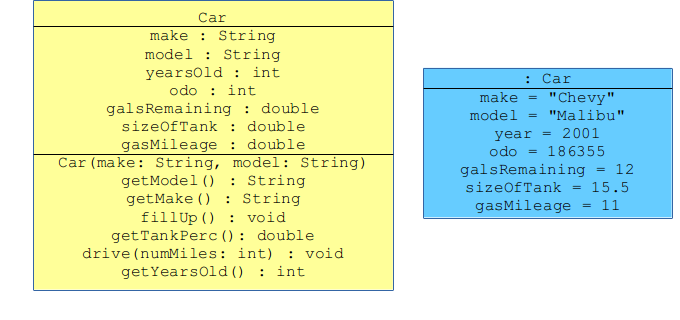
\includegraphics[width=1.0\textwidth]{classObject.pdf}   % 650x350
\caption{A class (left) and an object in UML.}
\label{fig:classObject}
\end{figure}

\subsection{Classes in UML: the first two compartments}

\index{capitalization}
Let's look at the class in detail. In the top box is its name; so far so good.
One thing to point out, though, is that in Java, \textit{the names of all
classes are \underline{capitalized}.} Don't ever violate this rule, for
convention's and confusion's sake!

\index{instance variables (inst vars)}
The second compartment has the class's \textbf{instance variables}. You'll
hear people use other terms for these like like ``member variables'' and even
``class variables,'' but I strongly prefer instance variables (or ``inst
vars'' for short) and here's why: \textit{every instance of a class has its
own copy of its instance variables.} This truth is absolutely fundamental to
OOP, and it's worth re-reading that sentence again and again until it's part
of your core being. Declaring a plain-ol' variable like ``\texttt{int x;}''
creates a single storage location in which a value can be stored. But
declaring an \textit{instance} variable is a far-reaching choice that destines
every \texttt{Car} (or whatever) that will come about in the future to have
its own copy of that variable. It's our way of defining the very structure of
Cars in perpetuity.

One slight headache is that the UML syntax differs from Java's a bit: instead
of listing the variable's type and then its name, we reverse them, we use
a colon instead of a space, and we omit the semicolon. Otherwise, it's pretty
straightforward to interpret that second compartment.

\index{class variable}
\index{underlined}
\index{car@\texttt{Car}}
\index{static@\texttt{static}}
By the way, one important piece of syntax in that second compartment is an
\underline{underline}. If an inst var is underlined, then it actually isn't an
``instance variable'' after all: it's a \textbf{class variable}. This means
that \textit{there's only one shared variable for the entire class, rather
than a different variable for each object.} In Figure~\ref{fig:classObject},
the integer \texttt{num} variable is the only underlined one. So even though
every \texttt{Car} has its own \texttt{make}, \texttt{model},
\texttt{odo}meter reading, \textit{etc.}, they all share one \texttt{num}
(which presumably represents the total number of \texttt{Car} objects
instantiated so far.) This makes sense, since after all such a variable is not
specific to a certain \texttt{Car}. We'll see that in Java, class variables
are created by using the ``\texttt{static}'' keyword where the variable is
declared.

\subsection{Classes in UML: the third compartment}

\index{method}
\index{member function}
The third compartment isn't much harder: it contains the \textbf{methods} for
the class. Like everything it seems, programmers have multiple terms for these
two: they're called \textbf{member functions} or \textbf{class functions} on
occasion. We'll stick with \textbf{method}.

\subsubsection{Functions vs. methods}

\index{function}
The crucial distinction between a method and a regular ol' Joe function is
this: while you can simply call a function to trigger it, you must call a
method \textit{on an object}. In the example, we have a \texttt{fillUp()}
method defined on the \texttt{Car} class. Since it's not an ordinary function,
but rather an OO method, we must call it on a particular instance of a
\texttt{Car}. In Java code, this does \textit{not} work:

\begin{verbatim}
    fillUp();        // NOPE
\end{verbatim}

nor does this:

\begin{verbatim}
    Car.fillUp();    // NOPE
\end{verbatim}

Instead, one must call \texttt{fillUp()} like this:

\begin{verbatim}
    johnsMercedes.fillUp();     // Correct!
\end{verbatim}

where \texttt{johnsMercedes} is the name of a valid \texttt{Car} object,
previously instantiated.

Beginners sometimes view this as a syntactic nuisance. It is not. It is
fundamental to what your code \textit{means}. Conceptually, it makes sense to
have a particular car, and to fill it up. It does \textit{not} make sense to
say ``hey universe, fill up cars'' (which is what ``\texttt{fillUp()}'' seems to
say) nor to say ``hey Cars-in-general, fill yourself up'' (which is what
``\texttt{Car.fillUp()}'' seems to say).

\index{capitalized}
By the way, notice in the example I just gave, \texttt{johnsMercedes} is
\textit{not} capitalized. (The capital ``\texttt{M}'' in the middle doesn't
count; that's just an artifact of CamelCase, which is a way of making multiple
words easier to read.) This is \textit{always} true: in Java, object names
should always begin with a lower-case letter.

Back to the third compartment. You can probably tell that the stuff inside the
parentheses is arguments to the respective methods, with the same
name-first-then-type colon-syntax, and you can probably tell that after the
closing parenthesis, you have the return type of the function. All of this
looks vaguely Java-like, and that's because even though a UML diagram is
technically programming-language-independent, language-specific things like
\texttt{int} and \texttt{String} can't help but creep in in practice. Our
thoughts betray us.

\subsubsection{Various ``special'' methods}
\label{page:instantiateConstructor}

\index{constructor}
\index{void@\texttt{void}}
A few of those methods are worthy of special note. The first one listed,
called simply ``\texttt{Car}'', is a very special kind of method called a
\textbf{constructor} which we'll be talking about a lot. Here's an iron-clad
rule which is fundamental to much that follows: \textit{whenever an object is
instantiated, one of its class's constructors is called.} This happens
automatically; it's not something we have to do ourselves. (Java's syntax for
this, as we'll see, makes it kind of look like we're calling the constructor
ourselves, which is a mixed blessing.) In Java, there are two things that
``make'' a method a constructor: (1) it must have exactly the same name as the
class, and (2) it must have \textit{no} return type. (Note that ``no'' return
type is not the same as a \texttt{void} return type! I mean \textit{no return
type at all.}\footnote{If you mistakenly include a \texttt{void} before your
constructor when you write the code, it is officially no longer a constructor!
It's now just an ordinary method -- weirdly named the same as the name of the
class it's in -- which will not be automatically invoked at instantiation time
as a constructor should. I once had a nasty bug at the eleventh hour of a
software release because of this exact issue.})

By the way, just as a class can have multiple methods with the same name as
long as those methods have different argument lists, so it can have multiple
constructors subject to the same conditions. This is a very common practice,
although in this first example we have only one \texttt{Car} constructor.

\index{underlined}
\index{numCars@\texttt{numCars()}}
Also, just as in the second compartment, an \underline{underline} indicates
that the method ``goes with the whole class, not with each object.'' And just
as before, this implies the use of the \texttt{static} keyword. A
\texttt{static} method is essentially a function: \textit{i.e.}, you
\textit{don't} call it on an object. Instead, you just call it \textit{on the
class itself.} In the example above, \texttt{numCars()} method is
\texttt{static}, which means that you could write ``\texttt{Cars.numCars()}''
to retrieve the number of \texttt{Car} objects that have been instantiated to
that point. Static methods are quite rare, but they do arise occasionally, and
are always indicated with an underline.

\index{getter}
\index{setter}
\index{mutator}
\index{accessor}
The other methods I'll draw your attention to are the ones that begin with
``\texttt{get}''. People call these methods ``\textbf{getters},'' and all they
normally do is return the value of the instance variable in question. Often
one also has ``\texttt{set}'' methods to set the values of inst vars, although
our example doesn't have any of those. Btw, some people also call getters and
setters \textbf{accessors}, and sometimes specifically call setters
``\textbf{mutators},'' a term which always made me chuckle.

\subsection{Objects in UML}

\index{object}
\index{state}
Now let's examine the blue box in Figure~\ref{fig:classObject}, which
represents an object rather than a class. It has only two compartments, not
three. That's because there's no need (in most OO languages) to say anything
about an object's methods when focusing on the object: after all, the methods
are simply defined by the class, and are common to all instances of that
class. It is important, however, to specify the current \textbf{state} of the
object, which means the current values of all its instance variables. In the
picture, you can see that there is a \texttt{Car} object in memory
representing an old Chevy Malibu with a zillion miles on it and other
suboptimal features.

\index{names}
Perhaps the strangest thing about a UML object is the top compartment. Notice
that it says ``\texttt{:~Car}'' (``colon-Car''), which is not a typo. Here's
the sitch. The top compartment of a \textit{class} has the class's name, since
that's all there is to say about it. The top compartment of an \textit{object},
meanwhile, has the \textit{object's} name, followed by a colon and then its
class. Just like we said ``\texttt{make :~String}'' earlier, so here we can
say ``\texttt{johnsMercedes :~Car}''. Why, then, is
Figure~\ref{fig:classObject} missing the name before the colon? Because we've
chosen \textit{not to name this object in the diagram.} It's just ``a Car''
with certain properties, not a named Car. This may seem odd, but in fact 99\%
of the time we will do exactly this. And that's because bizarrely,
\textit{objects don't have names in Java}, even though it may seem at first
that they do.

More on that later. For now, just accept the fact that UML diagrams can depict
objects, and normally we don't choose to specify the object's name -- only its
type and its instance variable values.


\subsection{The value of ``design''}

\index{design}
\index{class diagram}
\index{blueprint}
Before we move on to implementation, take a step back for a moment and
consider the \textit{information} contained in that
Figure~\ref{fig:classObject}.

Suppose you were given the job to write a car maintenance tracking program,
and you were getting started figuring out how to accomplish that. I think
you'll agree that if someone handed you that diagram, it would be valuable
indeed. There's no code in it \textit{per se}, but a great deal of the work
has already been done for you! You already know what to name your class, the
names and types of all its constituent variables, and what methods its objects
should support. With that diagram alone, I'd say 70\% of the work has been
done. All it takes now is to convert that diagram into Java (or whatever
language you're working with), and flesh out the methods to do the right
thing. But the overall blueprint communicates a ton of information about
decisions that have already been made. Your structure is defined, and now you
just need to bust out a hammer and some nails.


\section{Classes in Java}

\index{class@\texttt{class}}
\index{java file@\texttt{.java} file}
\index{vim@\texttt{vim}}
In Java, every class is in its own file\footnote{Technically there can be
some exceptions to this, but don't worry about them now.} named the same as
the name of the class (including the capital letter) with a \texttt{.java}
extension. Operationally, we can use \texttt{vim} to create it and edit it:

\begin{verbatim}
$ vim  Car.java
\end{verbatim}

\index{package@\texttt{package} statement}
\index{import@\texttt{import} statement}
% TODO: *Do* we actually talk about "package statements" later?
The skeleton of any class file -- after the \texttt{package} and
\texttt{import} statements we'll talk about later -- is the class definition,
with curly braces:

\begin{Verbatim}[samepage=true,fontsize=\footnotesize,frame=single]
class Car {
    
}
\end{Verbatim}

\index{public@\texttt{public}}
You may be used to putting the word ``\texttt{public}'' before the word
\texttt{class} here. For now, we won't do this, and I'll encourage you to
ditch the habit of making classes \texttt{public} by knee-jerk reaction. As
we'll learn, you want to lean towards making things ``as private as possible''
until you have reason to do otherwise.

\subsection{Instance variables in Java}

\index{instance variables (inst vars)}
Instance variables go directly inside the class definition, and outside of any
method:

\begin{Verbatim}[samepage=true,fontsize=\footnotesize,frame=single]
class Car {
    String make, model;
    int yearsOld;
    int odo;
    double galsRemaining;
    double sizeOfTank;
    double gasMileage;    
}
\end{Verbatim}

\index{private@\texttt{private}}
You may be used to seeing the word ``\texttt{private}'' before each instance
variable, and I do applaud that practice. More on that later. For now, we'll
leave it off just because it's not necessary to compile. Realize that it's not
the word \texttt{private} that makes something an instance variable; rather,
it's the fact that it's defined directly inside the class, rather than within
a method.

\subsection{Constructors in Java}

\index{constructor}
Next on the diagram is our constructor. We put in the boilerplate to get us
started:

\begin{Verbatim}[samepage=true,fontsize=\footnotesize,frame=single]
class Car {
    ...

    Car(String make, String model) {

    }
}
\end{Verbatim}

and now for the first time we have to actually think.

A constructor, as I said, is automatically called whenever an object comes
into existence. This is our ``hook'' to set up the object for success when
methods are called on it later. Think of it this way: your constructor is
called whenever a new object is about to come off the assembly line and enter
the real world. Your job in the constructor is to do everything necessary to
make sure it's ready for prime time.

Often this will involve initializing the instance variables to reasonable
values. Sometimes it will include other things, like registering its existence
in some global repository of objects, or initializing a connection to a
network, or writing itself to a database. The key question to ask yourself is,
``what do I need to do to ensure this object is `legit' and doesn't break
anything when it's being used?''

\subsection{Analyze \texttt{this}}

\index{this@\texttt{this}}
In our case, initializing the instance variables are all we need to do in the
constructor. First, let's set the object's \texttt{make} and \texttt{model} to
what was passed:

\begin{Verbatim}[samepage=true,fontsize=\footnotesize,frame=single]
class Car {
    ...

    Car(String make, String model) {
        this.make = make;
        this.model = model;
    }
}
\end{Verbatim}
\normalsize

\index{Gosling, James}
If this is the first time you've seen the odd word ``\texttt{this}'' in a
program, have a good chuckle. What a weird word choice! But Gosling \&
Co.~chose this word to denote a central OO programming concept. The word
``\texttt{this}'' means one of two different things, and they both need to be
memorized:

\begin{enumerate}
\large
\itemsep.1em
\item Inside a \textit{constructor}, ``\texttt{this}'' means ``the object that is
currently being instantiated.''
\item Inside a \textit{method}, ``\texttt{this}'' means ``the object the
method was called on.''
\item[-.] (Anywhere else, ``\texttt{this}'' is illegal.)
\normalsize
\end{enumerate}

It's weird and meta and self-referential, but it's also necessary. There are
times when we need to have a name for ``the very object I'm `in' right now,''
and ``\texttt{this}'' is our (awkward) name to refer to that.

So in our constructor, when we say ``\texttt{this.make}'' we mean ``the
\texttt{make} instance variable of this very object that is in the process of
being birthed.'' We set that to the \texttt{make} argument that was passed to
the constructor. Ditto with \texttt{model}. Oftentimes, using \texttt{this} is
optional, but in the present case it's required because we named our argument
the same as the instance variable, and there has to be a way to distinguish
between the two.

\index{initialization}
Now for our other inst vars. Some of them make sense to be set to zero:

\begin{Verbatim}[samepage=true,fontsize=\footnotesize,frame=single]
class Car {
    ...
    Car(String make, String model) {
        this.make = make;
        this.model = model;
        this.yearsOld = 0;
        this.odo = 0;
        this.galsRemaining = 0.0;
    }
}
\end{Verbatim}

since brand new cars are in fact zero years old, have a 000000 odometer, and
have no gas in their tank (maybe). Zero values for the other two don't make
sense, however; brand new cars still have a gas tank of a certain size, and
they certainly get more than 0 mpg. For this example, I'm going to go with a
very limited notion of automotive properties:

\begin{Verbatim}[samepage=true,fontsize=\footnotesize,frame=single]
class Car {
    ...
    Car(String make, String model) {
        this.make = make;
        this.model = model;
        this.yearsOld = 0;
        this.odo = 0;
        this.galsRemaining = 0.0;
        
        if (make.equals("Chevy") || make.equals("GM")) {
            sizeOfTank = 21;
        } else {
            sizeOfTank = 13;
        }
        if (make.equals("Chevy") && model.equals("Malibu")) {
            gasMileage = 3;
        } else {
            gasMileage = 24;
        }
    }
}
\end{Verbatim}

I'm totally not bitter about my car's gas mileage, by the way.

\subsection{Methods in Java}

The other methods follow a similar syntactic pattern. But it's super important
to keep this truth in the front of your mind: \textit{because they are methods
(not functions), they are called \underline{on an object.}} That means that
you can refer to instance variables inside of them -- and when you do, you're
talking about \textit{the instance variables of the object the method was
called on.} Put another way, you're talking about the instance variables of
\texttt{this}.

\subsubsection{``Client code'' and thinking reactively}

When you write methods in an OO program, you have to think reactively, not
proactively. What I mean is this. When you write a procedural, old school
program, you're the one in control. You set the agenda. In your
\texttt{main()} you say, ``first do this, then do that; create these three
variables, perform a computation, and then print the result.''

We all learned how to program this way. But in OO, you kind of have to think
backwards from that. Writing a method isn't like calling it; instead of giving
orders, you're providing a service to whoever called you. So when you write a
method, you have to think, ``okay, some other part of the code is now calling
me, for reasons of its own. What do I do in response to that?''

\index{client code}
Our term for ``that other part of the code that is now calling me'' is
\textbf{client code} (or sometimes just ``a \textbf{client}.'') The word
``client'' is used in a lot of different ways in high-tech, but here we just
mean ``the code that wants to use a particular object.'' The word connotes a
respected customer, whom we want to treat well. Very well, some client code
calls one of our methods. How should we react?

\index{state}
Often we'll react by updating the object's \textbf{state} to reflect what
should happen to it as a result of the method being called. Sometimes we'll
produce (return) a value that is stored by the object in question or
computed on the fly. Other times we'll trigger some side effect, like printing
to the screen, writing to a database, or calling some \textit{other} method(s)
on the same or a different object.

\index{implement}
\index{fillUp@\texttt{.fillUp()}}
This is best seen through examples. Let's implement\footnote{The verb
\textbf{to implement} means ``to take a design and actually build it out.'' It
is a synonym for the verb \textbf{to code}.} the \texttt{.fillUp()} method
first. Don't think about Java; think about cars. If I fill up a car, what
happens?

Does the make or model or mileage change? Of course not: the amount of gas in
the tank does. And ``fill 'er up'' means to raise it to its maximum. The
correct implementation of \texttt{.fillUp()}, then, is simply:

\begin{Verbatim}[samepage=true,fontsize=\scriptsize,frame=single]
class Car {
    ...
    void fillUp() {
        galsRemaining = sizeOfTank;
    }
}
\end{Verbatim}

We could equally well have written this as:

\begin{Verbatim}[samepage=true,fontsize=\scriptsize,frame=single]
class Car {
    ...
    void fillUp() {
        this.galsRemaining = this.sizeOfTank;
    }
}
\end{Verbatim}

to make it explicit that we're talking about two instance variables here, and
assigning the value of one to the other. It's a matter of style.

In the same vein, we ask ourselves, ``suppose some client code asks me what
percentage full my tank is. What answer do I give them?'' The proper response
involves these same two inst vars and a little math:

\begin{Verbatim}[samepage=true,fontsize=\scriptsize,frame=single]
class Car {
    ...
    double getTankPerc() {
        return galsRemaining / sizeOfTank * 100;
    }
}
\end{Verbatim}

I chose to omit \texttt{this}, but again it's a personal choice.

Some methods are no-brainers:

\begin{Verbatim}[samepage=true,fontsize=\scriptsize,frame=single]
class Car {
    ...
    String getModel() {
        return model;
    }
}
\end{Verbatim}

If a client asks me what my model is, I tell them my model, duh. The same is
true for the other accessor methods.

\index{drive@\texttt{.drive()}}
Finally, what if a client instructs me to drive $n$ miles? How should my
internal state be adjusted to reflect that?

This is the most difficult one, and again it requires you to think about cars
rather than about Java. Mentally run through the variables we've chosen to
represent a car, and ask yourself which ones need to change, and how? You'll
realize that the odometer and the gas tank level are the two we need to
modify. When someone drives a car $n$ miles, the odometer needs to increase by
$n$ miles (else it ain't legal); also, the gas tank needs to be reduced by
$\frac{n}{m}$ gallons, where $m$ is the car's gas mileage in mpg. So here we
go:

\begin{Verbatim}[samepage=true,fontsize=\footnotesize,frame=single]
class Car {
    ...
    void drive(int numMiles) {
        double galsBurned = numMiles / this.gasMileage;
        this.galsRemaining = this.galsRemaining - galsBurned;
        this.odo += numMiles;
    }
}
\end{Verbatim}

This time, I did include the \texttt{this}'s where appropriate, since we also
have a couple of local variables involved and I wanted to be explicit. Our
math is a mix of function parameters, temporary variables, and permanent
attributes of the \texttt{Car}.


\section{Objects in Java}

\index{object}
We've now coded a class from the ground up (the complete code listing is in
Figure~\ref{fig:carClassCodePreExceptions}.) We did this so clients can
instantiate objects of that type and do something with them. Let's make a
simple \texttt{main()} method to do just that.

You'd be surprised how many beginning programmers try to drive 23 miles like
this:

\begin{Verbatim}[samepage=true,fontsize=\scriptsize,frame=single]
    public static void main(String args[]) {
        drive(23);    // WRONG!
    }
\end{Verbatim}

or this:

\begin{Verbatim}[samepage=true,fontsize=\scriptsize,frame=single]
    public static void main(String args[]) {
        Car.drive(23);    // equally WRONG!
    }
\end{Verbatim}

Yes you'll get compiler errors, but those errors reflect a deeper and more
fundamental misunderstanding. In OOP, you have to call a method \textit{on an
object}. Conceptually, nothing else makes sense. In real life you don't
``drive in general,'' and you don't ask ``automobiles in general'' to drive
you places. Instead, you have to drive \textit{a particular car} somewhere.
Here's how:

\begin{Verbatim}[samepage=true,fontsize=\scriptsize,frame=single]
    public static void main(String args[]) {
        Car minivan = new Car("Toyota","Sienna");
        minivan.drive(23);    // correct!
    }
\end{Verbatim}

\index{new@\texttt{new}}
\index{instantiate}
The keyword ``\texttt{new}'' is utterly crucial here. In Java, \textit{the only
way to instantiate an object is to use \texttt{new}}. It causes a fresh object
of the appropriate type to spring into existence, complete with memory to hold
its instance variables. And the appropriate constructor is called, of course,
to set that object up for prime time.

We got errors before because we didn't even \textit{have} a car to do anything
with. There was no memory set aside, no constructor called to set up the
object, nothing. We tried a shortcut, and that was madness. But now that we
know how to instantiate objects, we can do so to several and create a whole
new world, as in Figure~\ref{fig:wholeNewWorld} on
p.~\pageref{fig:wholeNewWorld}. All the code in that figure is legit, and
shows that our \texttt{Car} class has uses.

\begin{figure}[h]
\centering
\begin{Verbatim}[samepage=true,fontsize=\footnotesize,frame=single]
    public static void main(String args[]) {

        // The archaic Davies family vehicles
        Car minivan = new Car("Toyota","Sienna");
        minivan.setYear(2002);
        Car stephensLemon = new Car("Chevy","Malibu");
        minivan.setYear(2001);

        // Grammy lives in Colorado
        Car grammysCar = new Car("Lexus","ES");
        grammysCar.setYear(2018);

        // Caravan to Disneyworld -- whoo-hoo!  (Grammy's meeting us there.)
        minivan.fillUp();
        minivan.drive(500);
        stephensLemon.fillUp();
        stephensLemon.drive(500);
        System.out.println("The van is " + minivan.getTankPerc() + 
            "% full, while the chevy is " + stephensLemon.getTankPerc() +
            "% full.");
        grammysCar.drive(1899);  // a long way from Colorado
    }
\end{Verbatim}
\caption{A client \texttt{main()} program that uses the \texttt{Car} class.}
\label{fig:wholeNewWorld}
\end{figure}


\subsection{Printing an object}

One last thing before we bring this chapter to a close. Suppose we're
debugging our program, and we want to print out the values of various
variables to help us hunt down an error. Printing an \texttt{int} or other
standard type is straightforward:

\begin{Verbatim}[samepage=true,fontsize=\scriptsize,frame=single]
    int numEnchiladas = 3;
    System.out.println("The number of enchiladas is: " + numEnchiladas + ".");
\end{Verbatim}

and will produce a message like ``\texttt{The number of enchiladas is 3.}''
What happens, though, if we print out an \textit{object}, like a \texttt{Car}?
How can such a complex entity be reduced to a string of text?

Heck, let's try it:

\begin{Verbatim}[samepage=true,fontsize=\scriptsize,frame=single]
    Car porsche = new Car("Porsche","Carrera");
    porsche.setYearsOld(2);
    System.out.println("My car is: " + porsche + ".");
\end{Verbatim}

The output we get is:

\begin{verbatim}
   My car is: Car@4aa298b7.
\end{verbatim}

Whoa. The word ``\texttt{Car}'' is perhaps not surprising, but what's the rest
of that gunk?

\index{memory address}
It turns out that Java's default way of rendering an object as a
\texttt{String} is to concatenate the name of the class, an ``at'' sign,
followed by \textit{the memory address} in which it is stored. We'll talk much
more about memory in the next chapter. For now, just think of the memory
address as a unique number\footnote{Yes, it is indeed a number, despite the
fact that it has letters in it like '\texttt{a}' and '\texttt{b}'. It's
printed here in \textbf{hexadecimal}, which is a base-16 number system instead
of the base-10 system non-computer-science humans use.} that identifies the
object, like an SSN.

\begin{samepage}
\label{pg:toString}
\index{override}
\index{toString@\texttt{.toString()}}
The cool thing is, we can \textbf{override} this functionality at will, and
change the way \texttt{Car}s will be printed. Check it out. Create a method in
the \texttt{Car} class called \texttt{.toString()}. It must:

\begin{compactenum}
\itemsep.1em
\item be called exactly ``\texttt{.toString()}''.
\item take no argument.
\item return a \texttt{String}.
\index{public@\texttt{public}}
\item have the word \texttt{public} immediately before the return type. (We'll
talk a lot about what \texttt{public} means in future chapters. For now, it just has to
be there.)
\end{compactenum}
\end{samepage}

Here's one:

\begin{Verbatim}[samepage=true,fontsize=\scriptsize,frame=single]
    public String toString() {
        return "a " + yearsOld + "-year-old " + make + " " + model;
    }
\end{Verbatim}

We're assembling various aspects of the vehicle into a sensible, readable
string. Now, when we run \textit{the same code} as above, our output is this:

\begin{verbatim}
   My car is: a 2-year-old Porsche Carrera.
\end{verbatim}

Notice that we didn't explicitly ever call \texttt{.toString()}! Instead, we
just used a \texttt{Car} object in a context in which a \texttt{String} was
required, and Java faithfully called our method instead of the one that
generated the memory address. Pretty cool.

\texttt{inheritance}
This is actually our first foray into a really deep and powerful technique
called ``inheritance,'' about which much more will come in later chapters. For
now, just grasp the idea that Java lets us override its general behavior for
specific kinds of objects, which gives us tremendous power and flexibility.

\begin{figure}
\begin{Verbatim}[fontsize=\scriptsize,frame=single]
class Car {
    String make, model;
    int yearsOld, odo;
    double galsRemaining, sizeOfTank, gasMileage;

    Car(String make, String model) {
        this.make = make;
        this.model = model;
        yearsOld = 0;
        odo = 0;
        galsRemaining = 0;
        if (make.equals("Chevy") || make.equals("GM")) {
            sizeOfTank = 21;
        } else {
            sizeOfTank = 13;
        }
        if (make.equals("Chevy") && model.equals("Malibu")) {
            gasMileage = 3;
        } else {
            gasMileage = 24;
        }
    }

    public String toString() {
        return "a " + yearsOld + "-year-old " + make + " " + model;
    }

    String getMake() { return make; }

    String getModel() { return model; }

    int getYearsOld() { return yearsOld; }

    void setYearsOld(int x) { yearsOld = x; }

    void fillUp() {
        this.galsRemaining = this.sizeOfTank;
    }

    double getTankPerc() {
        double perc = galsRemaining / sizeOfTank * 100;
        return perc;
    }

    void drive(int numMiles) {
        double galsBurned = numMiles / gasMileage;
        galsRemaining = galsRemaining - galsBurned;
        odo += numMiles;
    }
}
\end{Verbatim}
\caption{A complete Java implementation of the \texttt{Car} class.}
\label{fig:carClassCodePreExceptions}
\end{figure}


\chapter{Memory matters}
\label{ch:memoryMatters}

This chapter is near and dear to my heart. The concepts here are vastly
undertaught by computer science educators today, and yet they are at the
epicenter of most intermediate students' understanding (or misunderstanding).
A failure to master this material slaps a hard ceiling on what you can
accomplish as a programmer. Successfully mastering it is the key to the next
level.

The key idea is that there are two ways of looking at a computer program. One
is to look at the static lines of code as they are written on a screen or on
paper. This is how novices think about programs: they look at the lines of
code, and ask themselves whether lines need to be added, removed, changed, or
moved.

\index{memory}
The other way is to think about what happens to the computer's \textbf{memory}
as the program runs, and how its variables and structure change as the program
unfolds. Whether they realize it or not, this is how all proficient
programmers think. It turns out that \textbf{the ``purpose'' of almost any line
of code is to change the contents of memory in a particular way.} The name of
the game is recognizing what impact on memory each line of code has -- and
conversely, what line of code is required to make a particular change to
memory.

\section{Memory diagrams}

\index{memory diagram}
\index{snapshot}
The focal point of this chapter will be the \textbf{memory diagram}, which
incorporates the UML object representations we discussed in
section~\ref{sec:UMLclasses}. A memory diagram depicts the contents of the
computer's memory at a \textit{snapshot in time.} At any given moment, as a
program is running, you could say ``Freeze!''\ and look at the memory diagram.
You'd see the exact state of the system at that moment.

\subsection{The stack and the heap}

\index{stack@the stack}
\index{heap@the heap}
\index{memory!statically-allocated}
\index{memory!dynamically-allocated}

A program's memory, it turns out, is divided into two realms with funny names:
``\textbf{the stack}'' and ``\textbf{the heap}.'' It is vital to understand the
difference between the two, and which one is used for what. The stack contains
\textbf{statically-allocated}, and the heap \textbf{dynamically-allocated},
memory. We'll unpack what all this means, but first let me show you a full list
of differences:

\small
\vspace{.2in}
\begin{tabular}{c|c}
\textbf{stack} & \textbf{heap} \\
\hline
statically-allocated & dynamically-allocated \\
\index{names}
holds named things & holds unnamed things \\
holds primitive types and references & holds objects\footnote{This is
true in Java, but C++ permits programmers to store objects on the
\textit{stack} as well as the heap. I will argue that's universally dumb, and
it's a large part of what makes programming in C++ difficult: you have to
account for that occurrence with a ton of tedious and error-prone
bookkeeping.} \\
\index{lifespan}
items have limited lifespan & items have unlimited lifespan\footnote{Not
completely unlimited, but things on the heap stick around as long as they're
needed, rather than evaporating at the end of their current function.} \\
\end{tabular}
\vspace{.2in}
\normalsize

This is best understood by example, and in fact can be illustrated with just a
small function:

\begin{Verbatim}[fontsize=\small,samepage=true,frame=single]
void illustration() {
    int year = 2018;
    Car minivan = new Car("Toyota","Sienna");
}
\end{Verbatim}

This teensy function, when it runs, produces memory contents as depicted in
Figure~\ref{fig:stackHeap1}. Let's go through it carefully.

\begin{figure}[ht]   % 590x220
\centering
\includegraphics[width=1\textwidth]{stackHeap1.pdf}
\caption{The stack and the heap.}
\label{fig:stackHeap1}
\end{figure}

\index{primitive type}
The first line of \texttt{illustration()} creates a simple integer variable
and sets it equal to 2018. Since an \texttt{int} is a \textbf{primitive
type}\footnote{If you've never heard this lingo, a ``primitive type'' is one of
the very basic lower-case Java variable types, like \texttt{int},
\texttt{double}, or \texttt{boolean}. Importantly, a primitive type is
\textit{not} an object.}, it is stored on the stack. ``On'' the stack should
make you think of layering items vertically on a surface. Before this line of
code executed, nothing existed in the program's memory at all, so the stack
was nothing but a bare floor (think of it as a horizontal line). Our first
variable goes right on top of that floor.

\index{reference variable}
\index{variable, reference}
There's a ton packed into that second line of code, so hold on to your seats.
The first thing to realize is that \textit{it encompasses both stack and
heap.} We have a named \textbf{reference variable} called \texttt{minivan},
which, as with all named things, goes on the stack (right on top of
\texttt{year}). A ``reference variable'' means a variable that has the ability
to reference (or ``refer to,'' or ``point to'') an object. However, the object
itself is created in the heap, because in Java that's where all objects live.
The word \texttt{new} is a ``heap word'': using it is the only way to make an
object at all, and therefore, the only way to make something on the heap.
Finally, to carry out the equals sign (``\texttt{=}'') in that line of code, we
draw an arrow from \texttt{minivan} to the object to indicate that's what it's
currently referring to.

%\subsubsection{(...a brief commercial...)}
%
%Now before we go any further, I want to \textit{\textbf{implore}} you that
%\textit{this stuff does actually matter.} It's tempting at this point to think
%that all this gibberish about stack and heap and whether something's on the
%left or right side of a diagram is irrelevant.  Nothing could be further from
%the truth. As soon as our example gets even moderately complicated, you will
%absolutely get the wrong answer if you conflate or confuse the two memory
%realms, or fail to keep their contents utterly in sync. Trust me on this.
%
%\subsubsection{(...okay, back to work...)}

\index{names}
Okay, now a head-scratcher. Look at Figure~\ref{fig:stackHeap1} again. What
would you answer if I asked you, ``what's the \textit{name} of that blue
object?''

If you're like 99\% of novice programmers (including myself, long ago), you
would confidently answer, ``\texttt{minivan}. Its name is \texttt{minivan}.''
That seems to make perfect sense. But unfortunately it is \textit{wrong}. The
truth is that \textit{the object has no name.}

Again, you may think I'm being pedantic. Let me demonstrate why I'm not.
Suppose we expanded our previous code with four more lines, as depicted in
Figure~\ref{fig:additionalCode}. Study it carefully.

\begin{figure}
\begin{Verbatim}[fontsize=\small,samepage=true,frame=single]
void illustration() {
    ...
    Car other = new Car("Ferrari","F355");
    Car t = minivan;
    minivan = other;
    other = t;
}
\end{Verbatim}
\caption{(Continuing the previous example.)}
\label{fig:additionalCode}
\end{figure}

\index{car@\texttt{Car}}
Let's deal with the first two of these lines. The first one creates a new
reference variable called \texttt{other} on the stack, and points it to a
brand new \texttt{Car} object (unrelated to our Toyota Sienna) in the heap.
Notice that unlike with the stack, I didn't carefully put the new \texttt{Car}
exactly on top of the first one. Instead, I just threw it in there helter
skelter. This is how the heap works, and in fact why it's called a ``heap'':
it's a disorganized mess of stuff that comes and goes in response to the
program's unpredictable needs. The stack is as tidy as the Library of
Congress; the heap is a teenage boy's room. Seems weird, but it turns out
things have to be that way.

The second line creates a new stack variable called \texttt{t} but
emphatically does \textit{not} create a new \texttt{Car} object. Let that sink
in deeply. Many programmers, upon seeing a line begin with ``\texttt{Car t =
...} would naturally assume that line is making a new \texttt{Car}. But it's
actually only creating another variable that has the \textit{potential} to
refer to a \texttt{Car}. And in fact, after the equals sign, we do point it to
a \texttt{Car}...but one of the ones we've already instantiated (namely, the
Sienna).

The result of executing these two lines is shown in
Figure~\ref{fig:stackHeap2}. Stare very carefully at that figure and mull over
each box and line. We have four named variables, three of which are of type
\texttt{Car}, and yet there are only \textit{two} \texttt{Car} objects because
we only executed two \texttt{new}'s. And two of our named variables --
\texttt{t} and \texttt{minivan} -- are pointing to \textit{the same object}.
This turns out to be okay. We'll have multiple references to the same object
all the time, and it's entirely healthy. What's critical not to miss is that
\texttt{t} and \texttt{minivan} are not referring to identical copies of the
\texttt{Car}, but literally \textit{the same \texttt{Car}}. If we were to
change the state of \texttt{t}'s \texttt{Car} by, say, increasing its odometer
instance variable, \texttt{minivan} would instantly experience the same
change. And that's because they \textit{are} the same. 

\begin{figure}
\centering
\includegraphics[width=1\textwidth]{stackHeap2.pdf}   % 620x230
\caption{After executing the first two lines of code
Figure~\ref{fig:additionalCode}.}
\label{fig:stackHeap2}
\end{figure}


Okay, now the punchline of this whole example. I'm going to complete the
bait-and-switch, just to prove I was correct back when I said ``the name of
that first blue box is \textit{not} \texttt{minivan}.'' Let's do the
\textit{second} two lines of code in Figure~\ref{fig:additionalCode}:

\begin{Verbatim}[fontsize=\small,samepage=true,frame=single]
    ...
    minivan = other;
    other = t;
\end{Verbatim}

The result of those two operations is to change what the \texttt{other} and
\texttt{minivan} variables are pointing to. Memory now looks like
Figure~\ref{fig:stackHeap3}. And so I ask you again: ``what's the
\textit{name} of that Toyota Sienna object?'' I think you'll agree that
\texttt{minivan} is most certainly \textit{not} its name. Two valid ways to
refer to it are \texttt{t} and \texttt{other}, both of which point to it. But
neither one is its name. Objects simply have no name.

Names are ephemeral, momentary: they're only used temporarily so we can get at
the stuff in the heap, which is ultimately what matters.

\begin{figure}
\centering
\includegraphics[width=1\textwidth]{stackHeap3.pdf}   % 620x230
\caption{Finally, after executing the rest of code
Figure~\ref{fig:additionalCode}.}
\label{fig:stackHeap3}
\end{figure}

\index{lifespan}
Let me conclude this example by explaining what I meant earlier about
``limited lifespans.'' After executing the ``\texttt{other = t;}'' line, we are
done with the function. It's time to return control to whoever called
\texttt{illustration()} in the first place. And at this point, all of our
named variables -- \texttt{t}, \texttt{other}, \texttt{minivan}, and even
\texttt{year} -- cease to exist. Their destiny was only to provide service
during the time that \texttt{illustration()} was being executed. 

But the stuff on the heap lives on after. Long after a function is completed,
the objects it may have created or changed have a presence that will affect
the behavior of other, future functions. In this case, since we weren't passed
any arguments and didn't return anything, our Toyota and Ferrari \textit{will}
actually peacefully go away. But in general there are meaningful, long-term
effects, and in the next section we'll see an example in action.

Most methods are just like this. They create a few named variables so they can
change the contents of the heap in some way, and then clean up their toys
and return with the heap thus changed. That is their \textit{raison d'etre}.
It's a short but happy life.


\section{Calling functions}

\index{function}
One thing our previous example didn't include was calling a function or
method. In this section, we'll see what happens to memory when we do this.
There will probably be a few eye-openers for you.

First, take a look at our code listing (Figure~\ref{fig:functionCode}). We'll
switch from an automotive domain to part of a baseball simulator.

\index{ballplayer@\texttt{Ballplayer}}
\begin{figure}
\centering
\begin{Verbatim}[fontsize=\footnotesize,samepage=true,frame=single]
class Simulator {
    public static void main(String args[]) {
        int year = 2018;
        String greeting = "Play ball!";
        Ballplayer oldGeezer;

        ArrayList yankees = buildDaTeam();
        int rosterSize = yankees.size();
    }

    static ArrayList buildDaTeam() {
        String name = "Yankees";
        int year = 1927;
        ArrayList team = new ArrayList();

        Ballplayer ruth = new Ballplayer("Babe Ruth");
        ruth.setUni(3);
        ruth.setPos("OF");
        Ballplayer gehrig = new Ballplayer("Lou Gehrig");
        ruth.setUni(4);
        ruth.setPos("1B");
        Ballplayer babe = ruth;
        babe.setUni(3);       // (Pointless, as it turns out.)
        babe.setPos("OF");    // (Pointless, as it turns out.)
        team.add(babe);
        team.add(gehrig);
        team.add(ruth);
        
        return team;
    }
}
\end{Verbatim}
\caption{Some code that calls a function.}
\label{fig:functionCode}
\end{figure}

Let's see how the memory diagram emerges line-by-line in response to the code
executing.

First, let's execute the first three lines of \texttt{main()} and
``Freeze!''\ the picture. The result of these lines is shown in
Figure~\ref{fig:bpStackHeap1}. There are three new things here worth
mentioning. First, notice that our \texttt{greeting} variable, although it is
a \texttt{String}-with-a-capital-S and therefore an object, is shown on the
\textit{stack}, just like the \texttt{int year} is. The reason for this is
that Strings are a kind of in-between case (between primitive types and
objects) -- they're neither fish nor fowl. Technically they're objects, but
Java actually treats them somewhat specially, and even has an inline syntax to
create what are actually instances, so it ends up making more sense to treat
them as primitive types on the stack. That's what we'll always do with
\texttt{String}s.

\begin{figure}   % 650x240
\centering
\includegraphics[width=.9\textwidth]{bpStackHeap1.pdf}
\caption{Memory contents after executing the first three lines of
\texttt{main()}.}
\label{fig:bpStackHeap1}
\end{figure}

\subsubsection{Null references and NPEs}

\index{null pointer (or reference)}
\index{null@\texttt{null}}
The next new thing is that bizarre symbol next to \texttt{oldGeezer}.
\textit{Whazzat?} If you look at the code listing, you'll see that we
declare a variable of type \texttt{Ballplayer} named \texttt{oldGeezer}, but
we never set it equal to a \texttt{new} instance, nor to anything else for
that matter. This means that \texttt{oldGeezer}, which as you'll recall is a
``reference variable'' (capable of referring to a \texttt{Ballplayer})
currently refers to \textit{nothing}. In Java, this is called a \textbf{null
reference} (or \textbf{null pointer}) and is indicated with the keyword
\texttt{null}. In fact, this line of code has exactly the same effect as the
one above:

\begin{Verbatim}[fontsize=\small,samepage=true]
    Ballplayer oldGeezer = null;
\end{Verbatim}

Some people prefer to be explicit like this. I don't care either way; just
realize that at this point, if you attempted to call \textit{any} method on
\texttt{oldGeezer}, like:


\begin{Verbatim}[fontsize=\small,samepage=true]
    Ballplayer oldGeezer = null;
    oldGeezer.strikeout();
\end{Verbatim}

\index{NPE (null pointer exception)}
you will then be hit with the most ubiquitous of all Java
run-time errors, the \textbf{null-pointer exception} (or ``\textbf{NPE}''):

\begin{Verbatim}[fontsize=\small,samepage=true]
Exception in thread "main" java.lang.NullPointerException
    at Simulator.main(Simulator.java:5)
\end{Verbatim}

This is quite reasonable behavior, if you think about it. What can Java do if
you try to ``call a method on an object'' but there \textit{is} no such object?
It can only throw up its hands, which it does here.

Remember: an NPE means \textit{you tried to call a method on an object, but
the variable name you called it on wasn't actually an object; it was}
\texttt{null}. The way to diagnose an NPE is to look at the line number it
gives you, and find the dot (``\texttt{.}'') (or dots) on that line. The
variable or expression to the \textit{left} of one of those dots is an
uninitialized, null reference. Guaranteed.

\subsubsection{Stack frames}

\index{stack frame}
\index{recursion}
The last new thing in Figure~\ref{fig:bpStackHeap1} is easy to miss: it's the
word \texttt{main()} off on the left-hand side of the diagram. What this means
is that \textit{all the variables to the right of it ``belong'' to the
\texttt{main()} function.} This group of variables, which goes with a
particular call to a function\footnote{Note carefully that a stack frame is
associated with each \textbf{\textit{call}} to a function, not each function.
This may seem pedantic, and it is...until we consider \textbf{recursion}. A
recursive function will call itself, which will call itself, which will call
itself...many times. \textit{Each call} to the function generates its own
stack frame, which is separate from all the others. This is how recursive
functions are able to work without clobbering the values of the variables
contained in previous, still-active calls.}, is called a \textbf{stack frame}.
The way a program works is this: every time a function is called, a new stack
frame is ``pushed'' on top of the stack (above a horizontal line that we'll
draw.) While we're in the function, \textit{Java can only see the variables in
that current stack frame.} The ones in \texttt{main()}'s stack frame, or any
other stack frame for currently-in-progress functions, are safely nestled away
to be resumed later, but they are not immediately available to the program.

This is exactly how it should be. If we call a function \texttt{foo()} from
within a function \texttt{bar()}, control transfers to \texttt{foo()}. Now how
could \texttt{foo()} possibly refer to \texttt{bar()}'s variables? Heck,
whoever wrote the code for \texttt{foo()} didn't even know it would be
\textit{called} from \texttt{bar()}! Any other function could have called it
just as well, in which case \texttt{bar()}'s variables wouldn't even exist.
All we know for sure is that \texttt{foo()} was called from ``somewhere,'' and
thus must work no matter what the context. If Java allowed us to talk about
variables in another stack frame, our function would instantly become
non-reusable; it would only make sense if called from some specific other
function. And that defeats most of the purpose of even having a function.

Okay, now the big moment. We run this line:

\index{buildDaTeam@\texttt{buildDaTeam()}}
\begin{Verbatim}[fontsize=\small,samepage=true]
        ArrayList yankees = buildDaTeam();
\end{Verbatim}

which calls the \texttt{buildDaTeam()} function and transfers control to it.

Hang on to your hats. A lot happens here. First, a \textit{new stack frame} is
created, labeled \texttt{buildDaTeam()} in the diagram to carefully
distinguish it from the other. Then, \texttt{buildDaTeam()} starts executing.
Let's do the first three lines. We create two new variables on the stack
(a \texttt{String} and an \texttt{int}). One of these (\texttt{year}) has
\textit{the same name} as a variable that was declared down in
\texttt{main()}. This is perfectly okay, and the two \texttt{year}s in fact
have nothing whatsoever to do with each other. As long as
\texttt{buildDaTeam()} has control, ``\texttt{year}'' means \textit{the top
year}, in \texttt{buildDaTeam()}'s stack frame.

\index{null@\texttt{null}}
\index{instantiation}
In the third line, we create our first heap object of the entire program. It
is created (as all objects are created) with the \texttt{new} keyword. This
newly instantiated thing is an \texttt{ArrayList}, and we'll draw it as
indicated in Figure~\ref{fig:bpStackHeap2}. It has some \texttt{contents},
which is a zero-based, array-ish list of references, each of which has the
potential to point to an object.\footnote{You may be more used to seeing
\texttt{ArrayList<Ballplayer>} instead of just plain \texttt{ArrayList}, which
actually is a better choice. When we declare something as type
``\texttt{ArrayList<Ballplayer>}'' we're saying ``Java, please prevent me from
storing anything in this \texttt{ArrayList} \textit{except}
\texttt{Ballplayer}s.'' See section~\ref{sec:generics} for more details.}
Currently none of them do so, and therefore the diagram shows the
\texttt{null} symbol for each.

\index{snapshot}
Freeze! The program's memory now looks like Figure~\ref{fig:bpStackHeap2}.
Run your eyeballs over it and make sure you understand every box and line.

\begin{figure}   % 650x400
\centering
\includegraphics[width=.9\textwidth]{bpStackHeap2.pdf}
\caption{Memory contents after calling the function and executing the first
three lines of \texttt{buildDaTeam()}.}
\label{fig:bpStackHeap2}
\end{figure}

\subsubsection{Object craziness}

Now for the next part of code listing~\ref{fig:functionCode}. These three
lines:

\begin{Verbatim}[fontsize=\scriptsize,samepage=true,frame=single]
        ...
        Ballplayer ruth = new Ballplayer("Babe Ruth");
        ruth.setUni(3);
        ruth.setPos("OF");
        ...
\end{Verbatim}

\index{instantiation}
instantiate a new \texttt{Ballplayer} object (on the heap, of course) and set
it to some initial values. You need a little imagination to envision what the
\texttt{Ballplayer} class does in response to these method calls, but only a
little: obviously it has a constructor that takes a \texttt{String} (the
player's full name) and a couple of accessor/mutator methods to set the
player's uniform number and position. 

We then do the same sort of thing again, for another player:

\begin{Verbatim}[fontsize=\scriptsize,samepage=true,frame=single]
        ...
        Ballplayer gehrig = new Ballplayer("Lou Gehrig");
        gehrig.setUni(4);
        gehrig.setPos("1B");
        ...
\end{Verbatim}

to get another one. Then, we do this:

\begin{Verbatim}[fontsize=\scriptsize,samepage=true,frame=single]
        ...
        Ballplayer babe = ruth;
        babe.setUni(3);       // (Pointless, as it turns out.)
        babe.setPos("OF");    // (Pointless, as it turns out.)
        ...
\end{Verbatim}

\index{new@\texttt{new}}
which you know by now does \textit{not} instantiate a new object. (After all,
there's no \texttt{new}.) Instead, the first line \textit{points the new
variable \texttt{babe} at the same object \texttt{ruth} is currently pointing
to.} Get very, very comfortable with the idea that except for primitive types,
``\texttt{=}'' in Java does not do anything resembling a ``copy'' operation. It
simply makes a reference variable refer to something else. So we now have
three variables of type \texttt{Ballplayer}, but only \textit{two}
\texttt{Ballplayer} objects.

Finally, we add these players to our \texttt{ArrayList}:

\begin{Verbatim}[fontsize=\scriptsize,samepage=true,frame=single]
        ...
        team.add(babe);
        team.add(gehrig);
        team.add(ruth);
        ...
\end{Verbatim}

Stare closely at all those crazy arrows in Figure~\ref{fig:bpStackHeap3} and
make sure you understand where they're all going and why. Our
\texttt{ArrayList} object, instead of showing \texttt{null} pointers, now has
each of its slots pointing to a particular \texttt{Ballplayer} object.
Elements 0 and 2 point to the \textit{same} object, of course, because we
added ``\texttt{babe}'' and later ``\texttt{ruth}'' and those two variables are
pointing to the \textit{same} object. (So we're cheating here, baseball-wise:
you can't actually have the same player twice in the lineup! This is just an
example.)

\begin{figure}   % 800x460
\centering
\includegraphics[width=1\textwidth]{bpStackHeap3.pdf}
\caption{Memory after all the object creation done in \texttt{buildDaTeam()}.}
\label{fig:bpStackHeap3}
\end{figure}

\subsubsection{``I shall return''}

And now, we're ready to polish off this bad boy.

\begin{Verbatim}[fontsize=\scriptsize,samepage=true,frame=single]
        ...
        return team;
    }
\end{Verbatim}

\index{return@\texttt{return}}
That ``\texttt{return}'' statement packs a wallop. When the function is
completed, two huge things happen. First, the function's stack frame
\textit{is entirely wiped out.} Like, off the face of the planet. Every single
variable in there is irrevocably deleted and never mentioned again.

\index{stack@the stack}
\index{heap@the heap}
When students first hear this, they're sometimes dismayed -- ``what's the
point of calling a function then, if every single thing it creates is erased?''
Ahhhh...but they're only thinking of the \textit{stack}, not the heap. The
heap-ish things that a function accomplishes \textit{do} live on, and as I
said earlier, they are the reason the function existed in the first place.
Almost all functions' sole job is to inspect or manipulate the heap in some
way.

\index{stack frame}
When I say the stack frame is wiped out, here's what's wiped out: (1) all the
named variables in the stack frame, (2) all the primitive type values in the
stack frame (green boxes), (3) all the arrows emanating from the stack frame's
reference variables, (4) the word on the side of the diagram that names the
function, and even (5) the horizontal line that separates it from the stack
frame below.

\index{lifespan}
The result is that the top stack frame gets vaporized, leaving
\texttt{main()}'s stack frame open to the outside air. And that is exactly
what we want, because it's \texttt{main()}'s turn to take over now. Note that
all the heap stuff is still there: objects on the heap have an unlimited
lifespan, you'll remember.

\begin{figure}   % 750x460
\centering
\includegraphics[width=1\textwidth]{bpStackHeapFinal.pdf}
\caption{What memory looks like when we reach the end of \texttt{main()}.}
\label{fig:bpStackHeapFinal}
\end{figure}

\index{return@\texttt{return}}
The other thing the \texttt{return} statement does, of course, is put the
function's return value in the proper place, just before it's nuked. In this
case, since our original line of code was:

\begin{Verbatim}[fontsize=\scriptsize,samepage=true,frame=single]
        ArrayList yankees = buildDaTeam();
\end{Verbatim}

it makes \texttt{yankees} refer to the object that was ``returned,'' namely the
\texttt{ArrayList} that the shortly-to-die \texttt{team} variable is pointing
to.

We run one more line of code just to show we can do something with the
returned object (``\texttt{int rosterSize = yankees.size();}'') and the final
result is as in Figure~\ref{fig:bpStackHeapFinal}. There's no record of us
having called a function at all -- \texttt{buildDaTeam()} simply did its job
dutifully and quietly, and \texttt{main()} gets to reap the result.

\subsection{Calling a function from a function}

\index{function}
\index{stack frame}
By the way, this point is probably obvious by now, but let me clarify anyway:
if you call a function, and that function \textit{itself} calls
\textit{another} function, the same thing happens. The second function gets
its own stack frame with its own variables, while both the first function and
\texttt{main()} both get put on pause. There are at that moment \textit{three}
stack frames. When the second function returns, its stack frame disappears and
the first function becomes active; and when the first function returns,
\textit{its} stack frame disappears and \texttt{main()} becomes active.

\index{stack@the stack!pushing on}
\index{stack@the stack!popping off}
The terminology we use to describe this is somewhat obscure: when we create a
new stack frame for a newly-called function we call it \textbf{pushing} a new
frame on the stack. When we return, and get rid of it, we call it
\textbf{popping} the frame off the stack. Push and pop are lingo you'll see in
Data Structures class, when a data structure called a ``stack'' is introduced.
That stack data structure is a more general category of memory management
technique, of which ``the stack'' of our present chapter is an example.

Anyway, this whole push-a-frame-every-time-you-call-a-method thing (and
pop-the-top-frame-every-time-you-return thing) is central to how any computer
program operates. It's how your program breathes.


\section{Calling methods}

\index{method}
\index{this@\texttt{this}}
The mechanics of calling a function are just the same as when calling a
method, except for one thing: \texttt{this}. It turns out that when you call a
method on an object, you're adding one more thing to the stack: a reference to
the object the method was called on. And that, of course, is precisely what
``\texttt{this}'' means.

\index{ballplayer@\texttt{Ballplayer}}
\index{batting average}
Let's pan over to a different part of our fictitious baseball simulator: the
\texttt{Ballplayer} class itself. Part of the code for it is in
Figure~\ref{fig:BallplayerCode}.\footnote{Apologies to non-baseball fans. All
you really need to understand this example is that in baseball, every batter
accumulates a number of ``at bats'' (chances to come to the plate and hit
against a pitcher) and a number of ``hits'' (times he/she actually hit the ball
and made it at least to first base). A player's ``batting average'' is the hits
over the at bats; it ostensibly tells you how likely (on a scale of 0 to 1)
that player is to get a hit if he/she bats.}

\begin{figure}
\begin{Verbatim}[fontsize=\scriptsize,samepage=true,frame=single]
class Ballplayer {
    String name, position;
    int uni, numHits, numAtBats;

    Ballplayer(String name) {
        this.name = name;
        numHits = 0;
        numAtBats = 0;
    }

    void strikeout() {
        numAtBats++;
    }

    void getAHit() {
        numHits++;
        numAtBats++;
    }

    double getBattingAverage() {
        return ((double) numHits)/numAtBats;
    }
    ...
}
\end{Verbatim}
\caption{Part of the \texttt{Ballplayer} class.}
\label{fig:BallplayerCode}
\end{figure}

\index{pitcher@\texttt{Pitcher}}
\index{face@\texttt{.face()}}
\index{KO (strikeout)}
We're going to have a different class for pitchers, since they have different
stats (see Figure~\ref{fig:PitcherCode}).\footnote{Here, we're going to model
each pitcher as having a ``\texttt{koDominance}'' (``KO'' is baseball lingo for
``strikeout,'' btw). This is a number between 0 and 1 indicating the
probability of overwhelming the batter with a strikeout without that batter
being able to do anything about it.} The only method we'll show on the
\texttt{Pitcher} class is \texttt{.face()}, which is where a pitcher ``faces''
(pitches to) a batter in our simulation. The result will either be strikeout
or a hit in our extremely simplified view of the baseball world.

\begin{figure}
\begin{Verbatim}[fontsize=\scriptsize,samepage=true,frame=single]
class Pitcher {
    String name, handedness;   // L or R
    int uni, numKos;
    double koDominance;        // between 0 and 1
    static java.util.Random rng = new java.util.Random();

    ...
    void face(Ballplayer batter) {
        double koRandNum = rng.nextDouble();
        double batterRandNum = rng.nextDouble();
        if (koRandNum < koDominance) {
            batter.strikeout();
            this.numKos++;
        } else {
            if (batterRandNum < batter.getBattingAverage()) {
                batter.hit();
            } else {
                batter.strikeout();
                numKos++;
            }
        }
    }
}
\end{Verbatim}
\caption{Part of the \texttt{Pitcher} class.}
\label{fig:PitcherCode}
\end{figure}

\index{static@\texttt{static}}
\index{random number generation}
\index{Random.nextDouble@\texttt{Random.nextDouble()}}
\label{Random}
One item of note is the \texttt{static} variable \texttt{rng}, which stands
for \textbf{r}andom \textbf{n}umber \textbf{g}enerator. It's an instance of
the \texttt{java.util.Random} class, which the Java API provides to roll
random numbers. Every time you call \texttt{.nextDouble()} on a
\texttt{Random}, it generates a new random number between 0 and 1. It makes
sense for this to be a \texttt{static} variable, since the random number
generator itself is an object that all objects will share and use.

\index{face@\texttt{.face()}}
The specifics of the \texttt{.face()} algorithm aren't important to
understand. What is important is what happens in memory as this method is
called. Let's say our \texttt{main()} has the code in
Figure~\ref{fig:showdownCode}. After executing all lines but the last one, we
have the picture in Figure~\ref{fig:pitcherStackHeap1}. Take a moment and
convince yourself it's correct in all details.

\begin{figure}
\begin{Verbatim}[fontsize=\footnotesize,samepage=true,frame=single]
    public static void main(String args[]) {

        Ballplayer joltinJoe = new Ballplayer("Joe Dimaggio");
        joltinJoe.setUni(5);
        joltinJoe.setPosition("OF");

        Ballplayer theSayHeyKid = new Ballplayer("Willie Mays");
        theSayHeyKid.setUni(24);
        theSayHeyKid.setPosition("OF");

        Pitcher bestOfAllTime = new Pitcher("Sandy Koufax");
        bestOfAllTime.setUni(32);
        bestOfAllTime.setHandedness("L");
        bestOfAllTime.setKoDominance(.5);

        bestOfAllTime.face(theSayHeyKid);
    }
\end{Verbatim}
\caption{A mighty showdown on the diamond.}
\label{fig:showdownCode}
\end{figure}

\begin{figure}
\centering
\includegraphics[width=1\textwidth]{pitcherStackHeap1.pdf}  % 750x350
\caption{The baseball simulator's memory immediately before executing the
\textit{last} line of \texttt{main()} (``\texttt{bestOfAllTime.face(theSayHeyKid)}'').}
\label{fig:pitcherStackHeap1}
\end{figure}


And now for the moment we've all been waiting for: the first pitch of a new
(fantasy) baseball season, in which Sandy Koufax, the greatest pitcher of all
time, will face down Willie Mays, quite possibly the greatest hitter of all
time. I can't stand the suspense!!

\begin{figure}
\centering
\includegraphics[width=1\textwidth]{pitcherStackHeap2.pdf}  % 750x450
\caption{Memory while on the last line of \texttt{.face()}.}
\label{fig:pitcherStackHeap2}
\end{figure}

Figure~\ref{fig:pitcherStackHeap2} shows how memory looks during this
thrilling matchup. We're inside the \texttt{Pitcher}'s \texttt{.face()}
method, and so it has its own stack frame as expected. But I want to draw your
attention to two crucial aspects of this diagram:

\begin{enumerate}
\itemsep.1em
\index{this@\texttt{this}}
\item First, notice we have a visitor. On the stack frame, in addition to the
other expected variables, is none other than ``\texttt{this}''. Realize that
\texttt{this} is really just a reference variable like any other. What does it
refer to? \textit{The object the method was called on}, of course. In this
case, it's Sandy Koufax. How do we know? Because we didn't
just say ``\texttt{face(theSayHeyKid)}'' but
``\texttt{\textit{bestOfAllTime.}face(theSayHeyKid)}''. So the object that
\texttt{bestOfAllTime} refers to will be pointed to by \texttt{this} while
we're inside the method. Ponder this deeply.

\item Second, recognize that the \texttt{batter} argument -- which is a
reference variable of type \texttt{Ballplayer} -- is referring to the
\textit{same} object that \texttt{theSayHeyKid} is pointing to back in
\texttt{main()}. It is emphatically \textbf{\textit{not}} a copy of the
object. That's critical, because otherwise our \texttt{.face()} method would
have no way of updating Willie Mays' stats as a result of this
confrontation.\footnote{If you learned these terms in 220, this point can be
equivalently stated as follows: ``Java uses \textbf{pass-by-reference} for
objects, not \textbf{pass-by-value}.'' (Java \textit{does} use pass-by-value
for \textit{primitive types}, as we've seen: \texttt{int}s and such have their
own presence on the stack, and so are \textit{copied} from stack frame to
stack frame.)}

\end{enumerate}

Drum roll, please, before we hear the announcer: \textit{``...and it's a
scorching four-seam fastball from Koufax: swing and a miss, strike three!''}
The way the random numbers turned out in this example, Koufax was so
overpowering that he struck out Mays without the latter having a fighting
chance. (See how \texttt{koRandNum} was less than Koufax's
\texttt{koDominance}, so he blew him away without the \texttt{else} statement
coming into play -- \textit{i.e.}, without Mays' batting prowess even having a
chance to shine).

Don't worry, Willie: maybe you'll get one of your 660 lifetime home runs next
time you're up to bat. Console yourself with this: a different ``Willie'' Hall
of Famer (Willie Stargell) once quipped, ``trying to hit against Sandy Koufax
is like trying to drink coffee with a fork.''


\begin{figure}
\centering
\includegraphics[width=1.05\textwidth]{pitcherStackHeapFinal.pdf}  % 780x350
\caption{The final memory picture. Note the changed inst vars!}
\label{fig:pitcherStackHeapFinal}
\end{figure}

\index{pass-by-value}
\index{pass-by-reference}
The last diagram of the chapter, Figure~\ref{fig:pitcherStackHeapFinal}, shows
the situation when we return to \texttt{main()}. It's important not to miss
the main point here: both objects (\texttt{Pitcher} and \texttt{Ballplayer})
have their stats updated as a result of this showdown. If you're coming from a
language like C++, which passes objects by value, you might be raising your
eyebrows right about now. Get used to it. In Java, passing an object to a
function/method makes \textit{that exact object} available to the
function/method, not a copy. And certainly \texttt{this} is a reference to the
very object the method was called on, not a copy of it. This turns out to be
almost always what we want.




\chapter{Blueprints: UML class diagrams}

We spent last chapter discussing the \textbf{dynamic} view of a program: what
happens to memory, step by step, as it unfolds. In this chapter, we'll switch
to a \textbf{static} view: long-term, what are the program's classes, methods,
and relationships between them?\footnote{The words ``dynamic" and ``static"
are ubiquitous in computer science, and mean a zillion different unrelated
things. For example, we've already seen the Java ``\texttt{static}" keyword,
and how it indicates class-level rather than an object-level ownership. We've
also hinted at the stack having ``statically-allocated memory" and the heap
being ``dynamically-allocated." These terms are \textbf{\textit{unrelated}} to
our use of the words in this chapter. At present, by ``dynamic" we mean ``the
contents of memory changing as the program runs"; and by ``static" we mean
``the consistent, permanent characteristics of a program, quite apart from how
it might be behaving at any moment, which include its classes, methods, and
associations."}

If there's a type of UML diagram that deserves the name ``blueprint," it's the
\textbf{class diagram}. Class diagrams depict a high-level, stable perspective
of a software system. When you want to figure out how a large OO program
works, or when you're tasked with implementing a system that someone else has
designed, the first thing you look at are its class diagram(s).

UML class diagrams contain a number of elements, each of which has a very
specific meaning. We'll cover each in turn.

\section{Classes}

Unlike memory diagrams, which depict objects, class diagrams contain classes
(duh). We've already seen what a single class looks like in
section~\ref{sec:UMLclasses} (\textit{e.g.}, the left side of
Figure~\ref{fig:classObject}.) Most class diagrams contain many such classes.
Recall that each class has three compartments, containing the class's name,
its inst vars, and its methods, in that order.

By the way, one flexible (yet slightly annoying IMO) aspect of UML is that it
allows \textbf{varying levels of detail}. In other words, on a particular
diagram, you may or may not want to show all the instance variables and
methods, because it may or may not be relevant to the purpose of that
particular diagram. Similarly, you may or may not want to show all the aspects
of each inst var or method; perhaps it's too early in the design process to
completely specify all the parameters and return types, for example. To
illustrate, all three pictures in Figure~\ref{fig:graceful} are legit
ways of representing the \texttt{Car} class. We can include as much or as
little detail as we please.

\begin{figure}[ht]
\centering
\includegraphics[width=1\textwidth]{graceful.pdf}   % 670x320
\caption{Three equally valid ways to draw the \texttt{Car} class on a class
diagram, depending on how much detail it makes sense to include.}
\label{fig:graceful}
\end{figure}

The reason I find this annoying, by the way, is that it's ambiguous. If you
see no inst vars in the second box, does that mean (a) that class \textit{has}
no inst vars, or (b) the designer didn't think it was relevant to include them
on this particular diagram? No way to really know.

\section{Associations}

Perhaps the most important bits of information on a class diagram are the
\textbf{association}s between classes. An association means that two classes
collaborate together in some way to achieve some larger purpose. It is
indicated on a class diagram by a line connecting the two classes. Different
types of lines represent different kinds of relationships between the classes.
It's important not to mix them up, because if you do, you're dictating
something incorrect to the programming team about how the classes are intended
to work.

\begin{figure}[ht]
\centering
\includegraphics[width=0.7\textwidth]{assocArrows.pdf}   % 350x200
\vspace{.2in}
\caption{Diagrammatic elements for different association types.}
\label{fig:assocArrows}
\end{figure}

\subsection{Dependency associations}

Figure~\ref{fig:assocArrows} shows some of the UML association arrows and
their meaning. (There are others we'll get to in future chapters.) The dashed
line with a crow's foot arrowhead is called a \textbf{dependency}, and is the
``weakest" of the association types. When I say weak, I mean that the
relationship between the two classes isn't as important, nor as permanent, as
with the other association types we'll discuss later.

A dependency between classes \texttt{A} and \texttt{B} can be thought of in a
couple of ways:

\begin{compactitem}
\item One or more methods of the \texttt{A} class will \textit{call methods
on} a \texttt{B} object.
\item The \texttt{A} class \textit{is dependent on the interface of} the
\texttt{B} class.
\end{compactitem}

The word \textbf{interface} -- like stack, heap, dynamic, static, and many
other computer science words -- has multiple meanings. We'll talk about the
Java \texttt{interface} keyword later in the book. For now, when I say
interface I mean \textit{those aspects of a class that a user of that type of
object can see.} This boils down to: the methods you can call on it, together
with their argument lists and return types. Specifically, the interface does
\textit{not} include the method implementations (the bodies of the methods),
nor the instance variables.

If you think about it, you'll realize why the above two bullet points are
actually equivalent. Suppose some class \texttt{A} method has this line of
code in it: ``\texttt{String s = B.scissorKick(15)}". Then clearly the code in
the \texttt{A.java} file is \textit{dependent} on the fact that class
\texttt{B} has a \texttt{.scissorKick()} method, and that it takes an integer,
and returns a \texttt{String}. If any of that ever changed in the
\texttt{B.java} file, then class \texttt{A} would be impacted.

\begin{figure}[ht]
\centering
\includegraphics[width=0.8\textwidth]{dependencyAssoc.pdf}   % 
\caption{Examples of dependency associations.}
\label{fig:dependencyExamples}
\end{figure}

The strange-looking words adjacent to the dependency arrows in
Figure~\ref{fig:assocArrows} go by the even stranger-sounding term
\textbf{stereotypes}. A stereotype in UML is an extra bit of information that
enhances part of a diagram (an association arrow, as here, or sometimes a
class, method, or other element) by making its meaning more precise.
Stereotypes are usually displayed enclosed by double-wakkas
(``$\ll$...$\gg$").

In the case of dependency associations, the stereotype ``$\ll$uses$\gg$" means
pretty much what a dependency always means: that the designer intends class
\texttt{A} to ``use" (\textit{i.e.}, get its hands on, and call method(s) on)
object(s) of class \texttt{B}. The ``$\ll$instantiates$\gg$" stereotype goes a
bit further, and implies that some method of \texttt{A} will
\textit{instantiate} \texttt{B} objects in addition to merely calling methods
on them.

The examples in Figure~\ref{fig:dependencyExamples} are from a Dungeons \&
Dragons type combat simulator. A \texttt{Battle} object represents a fight
between adventurers and monsters. While simulating this fight, a
\texttt{Battle} will make use of one or more \texttt{Die} (singular of ``dice")
objects to roll random numbers that determine the outcome. This is a
``$\ll$uses$\gg$" association, since \texttt{Battle}'s code now depends on
\texttt{Die}'s interface not changing.

Elsewhere in the program, wizards sometimes cast ranged spells, like fireballs
or lightning bolts, to damage distant enemies. In the simulator, a
\texttt{Wizard} object might therefore instantiate a \texttt{RangedSpell}
object to carry out this attack. Since somewhere in the \texttt{Wizard} class's
code there will be a ``\texttt{new RangedSpell()}" line, we say that
\texttt{Wizard} $\ll$instantiates$\gg$ \texttt{RangedSpell}.


\subsection{``Has-a" associations}

The next strongest type of association has a bizarre name: it's called
``\textbf{has-a}." We denote it with a solid arrow between classes, with a
crow's foot on one side or both.

When class \texttt{A} has-a class \texttt{B}, that is nearly always a signal
to the programmer that \texttt{A} should have an \textit{instance variable} of
type \texttt{B}.\footnote{Or perhaps a \textbf{collection} of \texttt{B}
objects rather than a single \texttt{B} object, as we'll see later in the
chapter.} In other words, not only does an \texttt{A} object call
methods on a \texttt{B} (as in the dependency association), but an \texttt{A}
object actually holds on to one (or more) \texttt{B} objects for the
long-haul.

Now in some cases, the ``has-a" verbiage makes perfect sense. If our Domino's
Pizza delivery manager application had a \texttt{Pizza} class and a
\texttt{Topping} class, it would be no-brainer to say that every
\texttt{Pizza} has-a \texttt{Topping}. It conjures up in our minds a picture
of containment, or ownership. Perfect. However, we also use this type of
association in cases where containment doesn't make sense at all.

For example, in the same application it would be quite sensible to say that
``every \texttt{Pizza} has-a \texttt{DeliveryCar}." But obviously the delivery
car isn't ``inside" the pizza in the same physical way that the toppings are
inside it. So what does it mean then?

\begin{figure}[ht]
\centering
\includegraphics[width=1\textwidth]{wrongRightHasA.pdf}   % 
\caption{The \textbf{wrong}, and \textbf{right}, way of visualizing a ``has-a"
association in Java.}
\label{fig:wrongRightHasA}
\end{figure}

The key is making sure you have the right mental model.
Figure~\ref{fig:wrongRightHasA} shows both the wrong, and the right, way to
envision a has-a relationship (at least, in Java). In memory, there is
\textit{no} ``containment" as in the left-hand (wrong) image. The
\texttt{Topping} object isn't enclosed inside the \texttt{Pizza}, or even
exclusively owned by it. It's simply pointed to by one of the \texttt{Pizza}
object's inst vars. The right-hand side of the figure is the correct one --
and I daresay it's not problematic at all to think of a \texttt{Pizza}
``having" a \texttt{DeliveryCar} in this way. All it really means is that a
\texttt{Pizza} object ``knows about" a \texttt{DeliveryCar}, which is the
particular car that's delivering it.

Another reason that the correct mental model of ``has-a" is important is that
it is possible, and even common, for the association to go \textit{both ways}.
We use the term \textbf{navigability} for the question ``which direction does
the arrow go -- from \texttt{A} to \texttt{B}, from \texttt{B} to \texttt{A},
or both?" When it goes both ways, we call it a \textbf{bidirectional}
association.

\begin{figure}[ht]
\centering
\includegraphics[width=1\textwidth]{bidirectional.pdf}   % 750x235
\caption{A bidirectional ``has-a," depicted on a class diagram (left) and a
memory diagram.}
\label{fig:bidirectional}
\end{figure}

An example is the left-hand side of Figure~\ref{fig:bidirectional}. Here, our
\texttt{Driver} class and our \texttt{DeliveryCar} class each know about the
other, and in fact each hold on to an instance variable of the other type. If
we viewed this \texttt{A}-having-an-instance-variable-of-type-\texttt{B} thing
as the \texttt{A} object \textit{enclosing} the \texttt{B}, we'd blow a fuse.
\texttt{A} would contain \texttt{B}, which would contain \texttt{A}, which
would contain \texttt{B}, which... That way madness lies. But notice that
nothing paradoxical happens at all in the corresponding memory diagram on the
right-hand side of the figure. Each object points to the other, so that a
\texttt{Driver} object knows which \texttt{DeliveryCar} he/she is driving, and
a \texttt{DeliveryCar} also knows which \texttt{Driver} is driving it. No
biggie.

Note, by the way, that the has-a arrow implies the existence of the inst var
\textit{all by itself}. The class diagram should \textit{not} contain a
duplicate copy of the inst var in its second compartment. That would be
redundant, and is considered an error (see Figure~\ref{fig:wrongHasA}).

\begin{figure}[ht]
\centering
\includegraphics[width=1\textwidth]{wrongHasA.pdf}   % 640x180
\caption{One wrong way to model an instance variable. The ``has-a" arrow
already indicates that every \texttt{Pizza} has-a \texttt{Topping}: the
extraneous \texttt{topping} entry in the \texttt{Pizza} class's second box is
redundant and incorrect.}
\label{fig:wrongHasA}
\end{figure}


\chapter{The Singleton pattern}

``Singleton'' always sounded to me like the name of some small American town,
maybe one where nobody ever gets married. But it's actually the name of our
first (and easiest) \textit{design pattern}, and the subject of this chapter.

\section{Design pattern}

You know how when you sit down to write some code, there are times when you
think, ``wait, I've written this before''? Programmer's d\'{e}j\`{a} vu is
commonplace, especially because certain tips and tricks end up working in
a lot of different settings. For instance, we've all seen this sort of thing:

\vspace{-.1in}
\begin{Verbatim}[fontsize=\small]
    int multiplyAllTogether(int arr[]) {
        product = 1;
        for (int i=0; i<arr.length; i++) {
            product = product * arr[i];
        }
        return product;
    }
\end{Verbatim}

and this:

\pagebreak
\begin{Verbatim}[fontsize=\small]
    boolean hasAtLeastOneFive(int arr[]) {
        for (int i=0; i<arr.length; i++) {
            if (arr[i] == 5) {
                return true;
            }
        }
        return false;
    }
\end{Verbatim}

and this:

\begin{samepage}
\begin{Verbatim}[fontsize=\small]
    int getIndexOfHighest(int arr[]) {
        highestSoFar = arr[0];
        index = 0;
        for (int i=1; i<arr.length; i++) {
            if (arr[i] > highestSoFar) {
                index = i;
                highestSoFar = arr[i];
            }
        }
        return index;
    }
\end{Verbatim}
\end{samepage}

\index{programming pattern@``programming pattern''}
I could go on and on. You might think of these as ``programming patterns.''
They're bite-sized, go-to solutions that can handle a myriad of common little
programming scenarios.

It turns out that the same is true of design. Certain motifs in how classes
collaborate with each other crop up again and again in different settings.
They're important enough that they've been identified, described, and named.

\index{design pattern}
\index{Gamma, Erich}
\index{Vlissides, John}
\index{Johnson, Ralph}
\index{Helm, Richard}
\index{gang of four@the ``Gang of Four''}
The people who first promoted the idea of \textbf{design patterns} were Erich
Gamma, John Vlissides, Ralph Johnson, and Richard Helm, who were thereafter
nicknamed ``The Gang of Four.'' (You'll hear many references in the software
development industry to a ``Gang of Four design pattern,'' sometimes
abbreviated ``GoF design pattern.'' This means one of the 21 named patterns
that appeared in their hugely influential 1994 book \textit{Design Patterns:
Elements of Reusable Object-Oriented Software}. It's a book highly worth
obtaining and reading.)

One thing that's great about this is that just by mentioning one of these
agreed-upon pattern names -- like ``Observer,'' ``Iterator,'' or ``Strategy'' --
every developer worth their salt will instantly conjure up in their mind the
mechanics of that particular pattern, and know immediately what kind of
problem it's intended to solve. It saves a lot of words trying to describe an
idea you know your fellow developer has seen before, if only you could get
them to realize what you're talking about.

In this brief chapter, we'll cover the simplest GoF pattern of all:
the \textbf{Singleton} pattern.

\section{The Singleton pattern}

\index{Singleton pattern}
\index{design pattern!Singleton}
The Singleton pattern is so simple it almost doesn't even deserve to be called
a pattern. But it is. And it's easy to figure out when it applies to your
situation: \textbf{a Singleton is used when you have a class for which you
only ever want to instantiate one object.}

If you think about it, this kind of situation is pretty rare. Clearly any
relevant program is going to need to instantiate lots of different
\texttt{Car} objects, or \texttt{Ballplayer}s, or \texttt{Professor}s. There
are occasions, though, when your class isn't so much a category as it is a
special, one-of-a-kind object. Here are some examples:

\begin{itemize}
\itemsep.1em

\index{printerManager@\texttt{PrinterManager}}
\item Part of your operating system may have a \texttt{PrinterManager} class
that controls sending documents to various printers. The code will create many 
\texttt{Printer} objects, and many \texttt{Document}s, but only one
\texttt{PrinterManager} which runs traffic control and routes print jobs to
available printers.

\index{database@\texttt{Database}}
\item Your website that collects information about classic rock 'n' roll
albums may have a \texttt{Database} class that represents the underlying data
storage. You might get multiple \texttt{Connection}s to it and instantiate
multiple \texttt{Query} objects to search it, but there's just one
\texttt{Database} as a point of contact.

\index{configuration@\texttt{Configuration}}
\item Most programs have some way of configuring them, usually by tweaking the
values of various configuration variables. Your program could have a
\texttt{Config\-uration} class from which the other software components can
fetch the values of the settings as needed. There needs to be only
\textit{one} \texttt{Configuration} object, since they will all share access
to a common set of settings.

\end{itemize}

\index{instantiation}
\index{global point of access}
The Singleton pattern does two things: (1) it ensures that only one
instantiation is possible, and (2) it provides a global point of access to
that one object, so that the rest of the code can get to it.

\section{Implementation}

Here's what a properly-coded Singleton pattern looks like. We'll use the
\texttt{Configuration} example from above:

\begin{Verbatim}[fontsize=\small,samepage=true,frame=single]
class Configuration {
    private static Configuration theInstance;
    
    public static synchronized Configuration instance() {
        if (theInstance == null) {
            theInstance = new Configuration(...);
        }
        return theInstance;
    }

    private Configuration(...) {
        ...
    }

    // The actual methods of the object. For Configuration, this
    //   might include something like:
    public String getParamSetting(String param) {
        ...
    }
}
\end{Verbatim}

\index{static@\texttt{static}}
\index{theInstance@\texttt{theInstance}}
Let's go through each part carefully. First, we have a
\textit{\texttt{static}} variable called ``\texttt{theInstance}''. Recall that
\texttt{static} here means ``goes with the class as a whole, rather than with
each individual object.'' The reason for this is \textit{the class itself will
be holding on to its one-and-only instantiated object.} This is one of the few
places we'll be using \texttt{static} stuff in this book, because we need to.
If \texttt{theInstance} were \textit{not} \texttt{static}, then the only way
to get a hold of \texttt{theInstance} would be to have an instance of
\texttt{Configuration} in the first place...which would defeat the purpose of
the pattern.

\index{private@\texttt{private}}
Note that \texttt{theInstance} is also marked \texttt{private}. This is
partially because of our rule ``all inst vars should always be private,
period,'' but also because making this variable accessible outside the class
would make the whole pattern collapse. Parts of the code that needed access to
the \texttt{Configuration} singleton instance would try to grab
\texttt{theInstance} and use it, but it might not have even been set to
anything yet!

\index{instance@\texttt{.instance()}}
Next, we have the \texttt{instance()} method. This method is also
\texttt{static}, so that it can be called on the \textit{class} rather than on
an object. And what does it return? A \texttt{Configuration} object...or
perhaps I should say, \textit{the} \texttt{Configuration} object since there's
only ever going to be one.

\index{public@\texttt{public}}
\index{package visibility}
\index{thread}
\index{multithreaded program}
Unlike \texttt{theInstance}, \texttt{instance()} is public. (Package-level
visibility is also an appropriate choice, depending on how wide your intended
users of this Singleton are.) This is part of the public interface of the
class, designed to be called by code external to the class. The other word on
the declaration line is probably foreign to you: it's called
\texttt{synchronized}, and its purpose is beyond the scope of this chapter.
Very briefly, ``\texttt{synchronized}'' prevents two different \textbf{threads}
of execution from entering the \texttt{instance()} method at the same time.
A \textbf{multithreaded program} is one that executes more than one flow of
control simultaneously, each with its own stack. It turns out that if more
than one thread was inside this method at the same time, we might accidentally
instantiate \textit{two} (or more) \texttt{Configuration} objects. For our
single-threaded programs this isn't an issue, but it's good practice to get in
the habit of making your Singleton \texttt{instance()} methods synchronized.

Now let's dive in to the code for \texttt{instance()}. It's very simple, as
you'll see: all it does is say ``if this is the first time anyone's ever
called me, go ahead and instantiate an instance of me, and remember it (in the
\texttt{theInstance} class variable). Then, return the one-and-only instance
of me to the caller, to use to their heart's content.''

\index{lazy instantiation}
This is called \textbf{lazy instantiation}: the only thing that will trigger
the one-and-only \texttt{Configuration} object being instantiated is the first
time any other part of the program calls \texttt{Configuration.instance()}. If
nobody ever does call it, then there won't ever be even one instance of this
class created. But assuming someone does, a new \texttt{Configuration} object
will be instantiated \textit{this time only}. From that point on, all the
subsequent times \texttt{Configuration.instance()} is called, that same object
will be returned.

\index{constructor}
\index{private@\texttt{private}}
Then we have the constructor. It can do anything that any constructor can do,
which varies widely depending on what kind of class this is. (For the
\texttt{Configuration} example, perhaps it looks at the filesystem for a
\texttt{.config} file, and if it exists, loads it and remembers all its
contents in instance variables.) The important point to emphasize here is that
\textit{the constructor must be \texttt{private}}). That's because if it
weren't private, any old schmo could just write ``\texttt{new
Configuration()}'' and get a \textit{second} instance of the class, which is
precisely what we want to avoid. Making the constructor \texttt{private} means
nobody is allowed to instantiate a \texttt{Configuration} object...except for
the \texttt{Configuration} class itself, which we saw in the
\texttt{instance()} method.


\section{Using the Singleton}

This pattern allows any other part of the code base to do things like:

\begin{Verbatim}[fontsize=\footnotesize,samepage=true,frame=single]
  String bgcolor = Configuration.instance().getParamSetting("backgroundColor");
\end{Verbatim}

Whenever we say ``\texttt{Configuration.instance()}'' we get back a
\texttt{Configuration} object. (Whether we realize it or not, it's the only
such object that will ever exist.) There's no need to set this to anything, or
to use the word \texttt{new}; we just say ``\texttt{Configuration.instance()}''
every time we need it.

\index{instance variable (inst var)}
Other than this scaffolding, the rest of your Singleton class can do anything
it wants. It will almost certainly have other (non-static) instance variables,
and other methods to carry out its evil deeds. The ``Singleton part'' is just
the \texttt{instance()} and \texttt{theInstance} members, together with the
private constructor.

\index{Factory pattern}
\index{design pattern!Factory}
Singleton is often used in conjunction with the Factory pattern, by the way,
which we will look at in a future chapter.

That's it. Told you it was easy! $\smiley$


\chapter{Java odds 'n' ends}

Before we continue our study of OOA\&D proper, let's look at a few
Java-specific idiosyncrasies which will be all up in our business soon enough.

\section{Garbage collection}

\index{garbage collection}
No, I didn't make that term up just to be funny. \textbf{Garbage collection}
is actually the official name for a Java feature which was super innovative at
the time, but which we now often take for granted.

\index{ball@\texttt{Ball}}
\index{play@\texttt{.play()}}
Consider the code for a \texttt{Ball} class given in
Figure~\ref{fig:ballCode}. When we run it, Java calls \texttt{main()}, which
calls \texttt{play()}. At the end of \texttt{play()}, right before it returns,
a memory diagram would look like Figure~\ref{fig:ballMemory}. Take a moment to
see if you agree with all the details.

\begin{figure}[ht]
\begin{Verbatim}[fontsize=\scriptsize,samepage=true,frame=single]
class Ball {
    private String color;
    private int airPressure;

    Ball(String color) {
        this.color = color;
        airPressure = 0;
    }

    void bounce() {
        System.out.println("Boing!!");
    }

    static Ball play(int numBalls) {
        ArrayList equipment = new ArrayList();
        Ball b;
        int i;
        for (i=0; i<numBalls; i++) {
            b = new Ball("red");
            b.bounce();
            equipment.add(b);
        }
        Ball basket = new Ball("orange");
        return basket;
    }

    public static void main(String args[]) {
        int x = 3;
        Ball myBall = play(2);
        System.out.println("My ball is " + myBall.color + ".");
    }
}
\end{Verbatim}
\caption{A class to illustrate the utility of garbage collection.}
\label{fig:ballCode}
\end{figure}

\index{stack frame}
At this moment, we have an active stack frame for the \texttt{play()} function
which contains five variables of various types. And we're getting ready to
return the reference variable \texttt{basket} back to \texttt{main()}, which
means that about a nanosecond from now \texttt{main()} will be assigning its
new \texttt{myBall} variable to point to that orange ball.

\begin{figure}[ht]
\centering
\includegraphics[width=1\textwidth]{ballMemory.pdf}    % 750x400
\caption{A snapshot of memory, taken just before the \texttt{play()} function
returns back to \texttt{main()}.}
\label{fig:ballMemory}
\end{figure}

\index{memory diagram}
Okay, now let's do it. We return to \texttt{main()}. As soon as we do, the
memory diagram looks like Figure~\ref{fig:ballMemory2}. Take a close look.
That second diagram is all correct, but something about it may strike you as a
bit weird; namely, there are three objects on the heap \textit{with nothing on
the stack referencing them}. The \texttt{myBall} variable dutifully points to
the orange ball that was returned, but the two red balls, and the
\texttt{ArrayList} that contained them, are now disembodied from everything
else. And in fact, they are effectively \textit{lost} to the program. There's
simply no way to reference them. 

\begin{figure}[ht]
\centering
\includegraphics[width=1\textwidth]{ballMemory2.pdf}    % 750x400
\caption{The state of memory right \textit{after} the return to
\texttt{main()}. Notice there are now three unreachable objects on the heap.}
\label{fig:ballMemory2}
\end{figure}

If you're unsure that there's truly no way, ask yourself this question: ``what
line of code could we write to (say) change one of the \texttt{Ball} object's
color from red to blue?'' The answer is: there is no possible line of code we
could write to do that. To even get off the ground we'd have to start with a
\textit{name}, and there is no name we could possibly use to get at either of
those red \texttt{Ball} objects.

\index{C++}
\index{memory leak}
Now with C++, a language that preceded Java by decades, this would be a bad
situation called (I kid you not) a \textbf{memory leak}. The memory the
program used to store those now-unreachable \texttt{Ball}s is now inaccessible
to the program, and what's worse, \textit{C++ doesn't realize that's the
case.} So those old objects just sit there, growing stale, occupying system
memory that could be used to store other things instead. The program never
realizes this, and so never reclaims that space. So the actual amount of
memory the program has available to it has effectively shrunk.

\index{delete@\texttt{delete}}
In C++, the only remedy for this situation is for the programmer herself to
keep track of which objects no longer have any stack references to them, and
to explicitly \texttt{delete} those objects. This is a delicate task: fail to
\texttt{delete} what is in fact delete-able and you'll have a memory leak;
eagerly \texttt{delete} what actually does have other references to it and
your program will crash when that memory is reused by something else writing
over the top of it. The whole situation is fraught with peril.

\index{garbage collection}
Enter Java, in 1995. Java featured \textbf{automatic garbage collection} which
outsourced the whole responsibility for this from the programmer to a special
Java background task called the \textbf{garbage collector}. Whenever the
garbage collector runs, it intelligently sifts through the contents of memory,
looking for junk that can't be legally accessed anymore anyway. Whenever it
finds such junk, it \textit{automatically} tells the memory manager that that
memory is no longer in use, and can therefore be repurposed the next time the
program requests some memory with \texttt{new}.

Automatic garbage collection is lit. It means that pictures like
Figure~\ref{fig:ballMemory2} aren't scary at all. Sure, we have three objects
in the heap that can't ever be reached, but the garbage collector will soon
run, figure that out, and reacquire that memory so it can be used again. All
this without the programmer having to think a thing about it. Memory leaks are
in principle a thing of the past.

\index{pacemaker}
\index{C++}
As with most good things, there are downsides too. One downside to Java's
approach is that the garbage collector thread decides to run ``any time it
darn well pleases.'' As developers, we don't ever tell Java to get off its
butt and take out the trash (although there is a way to suggest this); rather,
we just wait for it to run when it periodically thinks it needs to. This isn't
normally a problem, but it can be in mission-critial real-time applications
with absolute performance deadlines. Think of the software running on a
pacemaker, which is embedded in a human heart. The code \textit{must} respond
in a certain amount of time in order to trigger the heart to take its next
beat! Now if, during our pacemaker program's operation, the garbage collector
suddenly decided to run in order to clean up lost memory, it might be a
time-consuming operation in its own right. And our program could literally
skip a beat (or beat later than it should) while waiting for it to finish. In
situations like these, C++'s style of manual control does give us more
fine-tuned flexibility over when exactly the reclamation of lost memory
occurs. For most applications, though, we don't need that flexibility and
Java's way of handling it is much appreciated.

\section{The \texttt{import} statement}

\index{import statement@\texttt{import} statement}
\index{include@\texttt{\#include}}
You've probably used \texttt{import} in almost every Java program you've ever
written. Yet I've found most developers don't really understand what it does.
Java itself is partially to blame here: the word ``import'' was a poor choice
for this, since nothing is ``imported'' at all.\footnote{Also, the fact that
it begins with a lower-case \texttt{i} just like C++'s ``\texttt{\#include}''
statement reinforces this misconception -- C++'s \texttt{\#include} actually
\textit{does} include/import content.}

Here's a statement that surprises a lot of Java programmers: you can write
\textit{any} Java program -- even one that uses stuff in the Java API --
\textit{without} an \texttt{import} statement. The left side of
Figure~\ref{fig:dontNeedImport} is such a program.

\begin{figure}[ht]
\begin{Verbatim}[fontsize=\scriptsize,samepage=true,frame=single]
                                                  import java.util.ArrayList;

class YouDontNeedImport {                         class YouDontNeedImport {                                                 
  public static void main(String args[]) {          public static void main(String args[]) {
    java.util.ArrayList celebs =                      ArrayList celebs =
      new java.util.ArrayList();                        new ArrayList();
    celebs.add("Kim Kardashian");                     celebs.add("Kim Kardashian");
    celebs.add("Justin Bieber");                      celebs.add("Justin Bieber");
    celebs.add("Taylor Swift");                       celebs.add("Taylor Swift");
    printEm(celebs);                                  printEm(celebs);
  }                                                 }
                                                
  static void printEm(java.util.ArrayList l) {      static void printEm(ArrayList l) {
    for (int i=0; i<l.size(); i++) {                  for (int i=0; i<l.size(); i++) {
      System.out.println("People love "                 System.out.println("People love "
        + l.get(i));                                      + l.get(i));
    }                                                 }
  }                                                 }
}                                                 }
\end{Verbatim}
\caption{The same Java program, using explicit inline package names (left),
and the \texttt{import} statement (right).}
\label{fig:dontNeedImport}
\end{figure}

No \texttt{import} required. Instead, on the left-hand side of the figure,
every time we want to refer to the \texttt{ArrayList} class, we specified it
as \texttt{java.util.ArrayList}. That does require us to type out the full
name three times, but it turns out to be all Java needs to understand
perfectly which \texttt{ArrayList} class we want to use.

Now since programmers (myself included) are lazy, and want to avoid typing
when possible, the Java gods invented the \texttt{import} statement. The
\textit{only} thing it does is tell Java ``I don't really feel like typing out
\texttt{java.util.ArrayList} every time. That's a pain. So Java, please know
that when I type \texttt{ArrayList} in this file, I really mean
\texttt{java.util.ArrayList}.''

The right-side of Figure~\ref{fig:dontNeedImport} is exactly the same program,
but now using the \texttt{import} statement to avoid a little typing.

Whether the savings are worth it in any particular case is up to you. My point
here is just to demonstrate that the statement ``\texttt{import
java.util.ArrayList}'' does \textit{not} do anything remotely like ``go and
find the \texttt{ArrayList} code in the \texttt{java.util} package, and bring
it in here so I can use it.'' Nor is it true that ``unless you import that
class, you can't use it.'' Both are common Java myths.

\subsubsection{Don't \texttt{import *}}

By the way, you may have seen the use of ``\texttt{*}'' syntax, like this:

\begin{Verbatim}[fontsize=\small,samepage=true]
import java.util.*;
import com.google.search.engines.*;
import edu.umw.stephen.coolclasses.*;
\end{Verbatim}

\index{scanner@\texttt{Scanner}}
This isn't a good idea. The reason is that it's ambiguous. Suppose in my code
I refer to a class called \texttt{Scanner}. Which \texttt{Scanner} do I mean?
Should Java assume I wanted to avoid typing ``\texttt{java.util.Scanner}'' or
``\texttt{com.google.search.engines.Scanner}'' or
``\texttt{edu.umw.stephen.coolclasses.Scanner}''? It has no way of knowing. So
if more than one of those packages defines a class with the same name (which
is very possible), Java will at best not compile, and at worst give unexpected
runtime behavior.

For this reason, using ``\texttt{*}'' in \texttt{import} statements is only
acceptable when writing quick and dirty one-off code, not for anything that
will stick around longer than your current coding session.



\section{Java ``generics''}
\label{sec:generics}

Speaking of misleading terms, let me give you another one.

There are two ways to use a container class from \texttt{java.util} (like
\texttt{ArrayList}, \texttt{Set}, or \texttt{PriorityQueue}). One way is to
just create one without any syntactic fuss:

\begin{Verbatim}[fontsize=\small,samepage=true,frame=single]
import java.util.ArrayList;
...
ArrayList stuff = new ArrayList();
\end{Verbatim}

and then put stuff in it:

\begin{Verbatim}[fontsize=\small,samepage=true,frame=single]
stuff.add("Laundry");
stuff.add("Lunchbox");
stuff.add(new Car("Mazda", "MX-5"));
\end{Verbatim}

\index{collection!heterogeneous}
\index{heterogeneous collection}
This is called a \textbf{heterogeneous} collection, because the things it
contains are of different types (\texttt{String}s and \texttt{Car}s, this
case).

\index{cast}
\index{typecast}
\index{downcast}
Java allows this perfectly well, for reasons we'll understand in detail later.
Here's the rub, though: when we get something \textit{out} of the collection,
we have to \textbf{cast} (or \textbf{typecast}, or \textbf{downcast}) it to
the correct type before doing anything specific with it. This code, for
example, does \textit{not} compile:

\begin{Verbatim}[fontsize=\small,samepage=true]
// Doesn't work:
System.out.println("First item has " + stuff.get(0).length() +
    " letters.");
\end{Verbatim}

The reason is that we're calling \texttt{.length()} on whatever object happens
to be at position \texttt{0} of the list, and Java can't know for sure whether
that object will end up being a \texttt{String}, a \texttt{Car}, or something
else. In particular, it can't know that that object will even \textit{have} a
\texttt{.length()} method. So Java makes us do this:

\begin{Verbatim}[fontsize=\small,samepage=true]
// Works, due to explicit cast:
System.out.println("First item has " + ((String) stuff.get(0)).length() +
    " letters.");
\end{Verbatim}

This says, ``Java, I give you my word. I promise the thing at position
\texttt{0} \textit{will} be a \texttt{String}, and I'll stake my reputation on
it. Please force it to be treated as a \texttt{String}, and if it turns out
I'm lying, you have permission to embarrass me at runtime with a program
crash.''

\index{generics}
Having to do that is a rather high price to pay for the flexibility of being
able to store any old thing in \texttt{stuff}. That's why back in 2004, Java
introduced the idea of \textbf{generics}, which allow you to restrict a
collection to having only items of a single type. Here's how you do it:

\begin{Verbatim}[fontsize=\small,samepage=true]
import java.util.ArrayList;
...
ArrayList<String> stuff = new ArrayList<String>();
stuff.add("Laundry");
stuff.add("Lunchbox");
stuff.add(new Car("Mazda", "MX-5"));    // Compile error
\end{Verbatim}

Our \texttt{stuff} is no longer a plain old \texttt{ArrayList}, but
specifically an \texttt{ArrayList<String>} (pronounced ``array list of
strings.'') This tells Java, ``please don't let me put anything into this
\texttt{ArrayList} \textit{except} \texttt{String}s. I'm asking for this
restriction because it's for my own good.''

When we do this, trying to insert a \texttt{Car} (or anything else) will bomb
at compile time, as it should. And now, we don't have to typecast anything we
get out of it: since Java knows it would only have put \texttt{String}s in, it
knows that it will only get \texttt{String}s out. Therefore,
``\texttt{stuff.get(0).length()}'' works just fine, no cast necessary.

This is a good feature, and you should pretty much always use it. My only
complaint is that I think the word ``generic'' is exactly the wrong word for
it. They almost couldn't have chosen a worse term. Saying you have ``a generic
\texttt{ArrayList}'' sounds like it ought to mean the \textit{first} style
(above), where the type wasn't specifically mentioned and therefore any object
was fair game to put in it. But in actual fact, ``a generic
\texttt{ArrayList}'' means ``a specific, decidedly \textit{non}-generic
\texttt{ArrayList} that is declared to only hold values of a certain type.''
Go figure.

\section{``Wrapper'' classes}

\index{pass-by-value}
\index{pass-by-reference}
This is a good time to explain the usage of Java's \textbf{wrapper} classes.
Recall that there are two kinds of Java variables: those that store primitive
types (like \texttt{int}) and those that refer to objects (like \texttt{Car}).
The biggest practical difference between these two, as we've seen, is where
they're stored: primitive types go on the stack (and hence are pass-by-value)
whereas the objects pointed to by reference variables go on the heap (and
hence are pass-by-reference).

\index{primitive type}
Another difference relates to the container classes like \texttt{ArrayList}
that we've just been discussing. All those \texttt{java.util} goodies, it
turns out, can store any type of object...but it must be exactly that: an
\textit{object}. In particular, they can't store primitive types.

So this means we can't do this:

\begin{Verbatim}[fontsize=\small,samepage=true]
    import java.util.ArrayList;
    ...
    ArrayList<int> uniformNumbers = new ArrayList<int>();     // NOPE
\end{Verbatim}

because there's no such thing as ``an \texttt{ArrayList} of \texttt{int}s.''
That sucks because \texttt{int}s, \texttt{double}s, and \texttt{boolean}s are
things we'd like to make \texttt{ArrayList}s of all the time.

\index{wrapper class}
Fortunately, there's an easy way around this. Each primitive type has a
``wrapper class'' in Java: it is the mold for objects so simple that they don't
do anything except hold a piece of data: an \texttt{int} (or \texttt{char}, or
\texttt{double}, \textit{etc.}) We could do this, for instance:

\begin{Verbatim}[fontsize=\small,samepage=true]
    Integer michaelJordan = new Integer(23);
    Integer derekJeter = new Integer(2);
    Boolean gameOfThronesRocks = new Boolean(true);
\end{Verbatim}

and produce the memory diagram in Figure~\ref{fig:wrapper}. Each object is
nothing more than a shell that ``wraps'' a primitive piece of data.

\begin{figure}[ht]
\centering
\includegraphics[width=0.8\textwidth]{wrapper.pdf}  % 650x250
\caption{Wrapper objects live on the heap.}
\label{fig:wrapper}
\end{figure}

So far this isn't very exciting. But one reason we need it is so we can store
primitive types in container objects like \texttt{ArrayLists}s. Here's all we
need to do to create our list of uniform numbers:

\begin{Verbatim}[fontsize=\small,samepage=true]
    import java.util.ArrayList;
    ...
    ArrayList<Integer> uniformNumbers = new ArrayList<Integer>();
\end{Verbatim}

and it works, since the elements of the \texttt{ArrayList} are declared to be
objects, as required. (Really teensy-tiny objects that don't really do
anything, but objects nonetheless.)

It's nice that after this, Java lets us work with primitive variables rather
than the wrapper classes:

\begin{Verbatim}[fontsize=\small,samepage=true]
    uniformNumbers.add(23);
    uniformNumbers.add(2);
    uniformNumbers.add(20);
    int mikeSchmidt = uniformNumbers.get(2);
\end{Verbatim}

so we really only notice the wrapper part at instantiation time. This isn't
the only time we need to use wrappers, but it's the only one we need in the
immediate future.

\section{The \texttt{Hashtable} data structure}

\index{hashtable@\texttt{Hashtable}}
\index{dictionary}
\index{Python}
\index{key-value pair}
One very, very common container type that we'll use is
\texttt{java.util.Hashtable}. (If you've used a \textbf{dictionary} in Python,
this is essentially the same thing.) A \texttt{Hashtable} holds a container of
\textbf{key-value pairs}. Each key-value pair represents a \textit{named}
piece of data -- the key is the name, and the value is the data. So unlike an
\texttt{ArrayList}, where the data elements are numbered, and thus accessed by
a numerical index, a \texttt{Hashtable} uses the keys to specify which piece
of data is required.

\index{alterEgos@\texttt{alterEgos}}
An example will make this all clear. Suppose we want to keep track of
superheroes and the names of their secret identities, so that if the
government decides to legislate against super powers, we can hunt down all the
potential perpetrators. We'll do so in a \texttt{Hashtable} called
\texttt{alterEgos}:

\index{Batman}
\begin{Verbatim}[fontsize=\small,samepage=true,frame=single]
    import java.util.Hashtable;
    ...
    Hashtable<String,String> alterEgos = new Hashtable<String,String>();
    alterEgos.put("Superman","Clark Kent");
    alterEgos.put("Batman","Bruce Wayne");
    alterEgos.put("Elastigirl","Helen Incredible");
\end{Verbatim}

\index{instantiation}
This instantiation syntax may make you bug-eyed. You'll see that we include
not one but \textit{two} types inside the ``$\ll...\gg$'' markers; in this
case, both are \texttt{String}s. These two specify \textit{the type of the
keys, and the type of the values}. Since our keys are text (superhero names)
and our values are also text (the names of the alter egos) it makes sense to
make this a \texttt{String}-to-\texttt{String} hash table.

\index{put@\texttt{.put()}}
The \texttt{.put()} method is used to add a new key-value pair to the table.
It is also used to \textit{change} the value that goes with a particular key.
That works because in a hash table, \textit{every key goes with just one
value}. If we ran a line of code like this:

\begin{Verbatim}[fontsize=\small,samepage=true,frame=single]
    alterEgos.put("Batman","Rich Dude");
\end{Verbatim}

then the \texttt{String} ``\texttt{Bruce Wayne}'' would be permanently removed
from memory, and replaced by ``\texttt{Rich Dude}''.

To retrieve the value that goes with a particular key, we use \texttt{.get()}:

\begin{Verbatim}[fontsize=\small,samepage=true,frame=single]
    String elastigirlTrueIdentity = alterEgos.get("Elastigirl");
    System.out.println("Pssst...Superman is really: " + 
        alterEgos.get("Superman"));
\end{Verbatim}

This looks very much like the way we obtain items from an \texttt{ArrayList},
except for \texttt{ArrayList.get()} we passed an integer, and for
\texttt{Hashtable.get()} we pass a key (whatever type that may be).

A very common use of \texttt{Hashtable}s is to store objects based on some
kind of name or identifier. For example:

\index{customer@\texttt{Customer}}
\begin{Verbatim}[fontsize=\footnotesize,samepage=true,frame=single]
    import java.util.Hashtable;
    ...
    Hashtable<Integer,Customer> customers = new Hashtable<Integer,Customer>();
    ...
    customers.put(7533, new Customer("Joe Blow", "New Plymouth, ID"));
    customers.put(6717, new Customer("Jill Hill", "New York, NY"));
    ...
    Customer custNum6717 = customers.get(6717);
\end{Verbatim}

Here we're storing \texttt{Customer} objects by their customer ID numbers, for
easy retrieval by that later.

In this book, I'll draw \texttt{Hashtable} objects as shown in
Figure~\ref{fig:hashtable}. Its \texttt{contents} table is full of references:
each box in the left column points to a key (in this case, an
\texttt{Integer}) and the box to its immediate right points to the
corresponding value (a \texttt{Customer}). Notice that there is no
well-defined order to the entries in the table -- in this case, even though
\texttt{Joe Blow} was the first one inserted, he occupies the second row of
the table. This is to emphasize that when you add a key-value pair to a
\texttt{Hashtable}, it doesn't remember anything about when you added it, only
that you \textit{did} add it.

\begin{figure}[ht]
\centering
\includegraphics[width=1\textwidth]{hashtable.pdf}
\caption{A \texttt{Hashtable} of \texttt{Customer} objects, stored by their
customer IDs.}
\label{fig:hashtable}
\end{figure}

\subsection{Iterating through \texttt{Hashtable}s}

\index{iteration}
One last thing about \texttt{Hashtable}s: you can iterate through them as you
can iterate through any other collection (like an \texttt{ArrayList}). But
it's kind of tricky. Remember that there isn't any inherent ``order'' to the
key-value pairs, so you can't say ``give me the first one, then the second,
then ..., all the way to the end.''

\index{enumeration@\texttt{Enumeration}}
\index{design pattern!Iterator}
\index{Iterator pattern}
The way you achieve this is by using an \textbf{\texttt{Enumeration}} object,
also from the \texttt{java.util} package. This is actually an example of the
\textbf{Iterator} design pattern, which we'll see in a later chapter. For now,
mostly just memorize the approach.

\index{keys@\texttt{.keys()}}
\index{nextElement@\texttt{.nextElement()}}
First, you call \texttt{.keys()} on the \texttt{Hashtable} which returns an
\texttt{Enumeration} of the ``key halves'' of the key/value pairs. Think of an
\texttt{Enumeration} as just ``a way to iterate through a group of things, one
by one.'' In this case, the ``things'' are the \texttt{Hashtable}'s keys. Every
time you call \texttt{.nextElement()} on the \texttt{Enumeration} object, it
gives you the next key and advances the ``cursor'' to point further on down the
line. When you call \texttt{.hasMoreElements()} on the \texttt{Enumeration},
it tells you whether or not you can continue further. These two methods are
just what you need to write a \texttt{while} loop to cycle through all the
keys; and each time you get a key, you can use the original \texttt{Hashtable}
to retrieve the corresponding value. To wit:

\begin{Verbatim}[fontsize=\small,samepage=true,frame=single]
    import java.util.Hashtable;
    import java.util.Enumeration;
    ...
    Hashtable<String,String> alterEgos = new Hashtable<String,String>();
    ...
    Enumeration<String> superheroNames = alterEgos.keys();
    while (superheroNames.hasMoreElements()) {
        String superheroName = superheroNames.nextElement();
        System.out.println(superheroName + " is really " +
            alterEgos.get(superheroName));
    }
\end{Verbatim}

Note how whereas the \textit{key} is retrieved directly from the
\texttt{.nextElement()} method, to get the \textit{value} we have to go back
to the \texttt{Hashtable} itself and call \texttt{.get()} with the key.

Also, remember that the order in which you're given the key-value pairs here
is \textit{not} necessarily the order in which you inserted them. That order
is irretrievable after the fact -- and if you need to keep track of it, you'll
need a separate data structure (perhaps an \texttt{ArrayList} of the keys, in
order of insertion) to remember it.

\section{Command-line arguments}

Every Java program you've ever written has this line in it:

\begin{Verbatim}[fontsize=\footnotesize,samepage=true,frame=single]
    public static void main(String args[]) {
\end{Verbatim}

\index{args@\texttt{args}}
Have you ever wondered what that ``\texttt{args}'' thing is for?

\index{command-line argument}
Like all programming languages, Java lets you access the \textbf{command-line
arguments} that the user typed after the program name when she ran the
program. Command-line arguments are nothing new for a budding Linux user. For
instance, this sort of command is second-nature to you by now:

\medskip
\quad \texttt{\$ cp \ Program1.java \ \freakingtilde/backup }
\medskip

It consists of a command name (``\texttt{cp}'') plus two command-line
arguments, which are: ``\texttt{Program1.java}'', and
``\texttt{\freakingtilde/backup}.''

Now it turns out that \textit{every} Linux program is capable of taking
command-line arguments, including Java programs. Suppose I type this:

\medskip
\quad \texttt{\$ java \ Simulator \ UMW \ Marymount}
\medskip

\index{main method@\texttt{main()} method}
As you know, this is a command to run a Java program whose \texttt{main()}
method is in \texttt{Simulator.java}. Apparently, the user is trying to
simulate a basketball game between two opponents, and is using command-line
arguments to specify which opponents. 

The only question that remains is: how does the Java code get access to those
strings that were typed on the command line when it was run? The answer is
\texttt{args}. When \texttt{main()} is called, \textit{Java passes the
command-line arguments to it as an array of Strings.} It's that simple. Inside
\texttt{main()}, you can treat the variable ``\texttt{args}'' in the same way
as any other array. For instance, if your code says:

\begin{Verbatim}[fontsize=\footnotesize,samepage=true,frame=single]
class Simulator {
    public static void main(String args[]) {
        System.out.println("There were " + args.length + " command-line args.");
    }
}
\end{Verbatim}

then the output, when run with the command above, will be:

\medskip
\quad \texttt{There were 2 command-line args.}
\medskip

And if your code says:

\begin{Verbatim}[fontsize=\footnotesize,samepage=true,frame=single]
class Simulator {
    public static void main(String args[]) {
        System.out.println("The first argument was: " + args[0] + ".");
        System.out.println("The second argument was: " + args[1] + ".");
    }
}
\end{Verbatim}

then the output, when run with the command above, will be:

\begin{Verbatim}[fontsize=\small,samepage=true,frame=none]
    The first argument was: UMW.
    The second argument was: Marymount.
\end{Verbatim}

This is powerful because it allows users to run your program with different
inputs and options \textit{without} having to recompile it (or even have
access to a compiler at all).

\section{Sameness vs.~identicality}

\index{sameness}
\index{identicality}
Our last odd/end has to do with how Java determines whether two objects are
``equal'' to each other. It turns out that there are two different definitions
of equality, which must be kept firmly separate in your mind:
\textbf{sameness} and \textbf{identicality}.

Consider the memory diagram in Figure~\ref{fig:sameness}. Here we have four
named variables: \texttt{p1}, \texttt{p2}, \texttt{p3}, and \texttt{p4}. Now
riddle me this, Batman: at the moment this snapshot was taken, which of these
variables do you consider to be \textit{equal} to each other?

\begin{figure}[ht]
\centering
\includegraphics[width=1\textwidth]{sameness.pdf}
\caption{What does ``equal'' mean?}
\label{fig:sameness}
\end{figure}

\index{equality}
I think we can agree that \texttt{p2} does not ``equal'' any of the others.
That leaves the other three. Are \texttt{p1} and \texttt{p3} ``equal?'' Are
\texttt{p3} and \texttt{p4} ``equal?''

It all depends on what your definition of ``equal'' is, of course. And here's
how Java does it: it says that \texttt{p1} and \texttt{p3} are \textbf{the
same}, while \texttt{p3} and \texttt{p4} are \textbf{identical}. ``The same''
means that the two reference variables refer to \textit{the very same} object
in memory. They are literally pointing to the same memory address, and so they
are pointing to the same ``copy'' of the object. This is easy to see by
imagining changes to that object -- if the left-most Josh Gibson changed
uniform numbers when he was traded from the Homestead Grays to the Pittsburgh
Crawfords, both \texttt{p1} and \texttt{p3} would automatically see that
change. They point to the same object, so they refer to the same uniform
number variable: if it changes, they both change.

But \texttt{p3} and \texttt{p4} are not the same -- they're merely identical.
They refer to two \textit{different} objects which just happen to have the
same internal state. Changing one would not affect the other. At the moment,
they're duplicate copies, but copies nevertheless.

(By the way, realize that sameness \textit{implies} identicality. The objects
\texttt{p1} and \texttt{p3} refer to the same, and therefore they are
\textit{also} identical.)

\subsection{Testing for sameness and identicality}

Sometimes a programmer cares about one of these conditions, and sometimes the
other. Java has two syntaxes to distinguish between the two tests.

\index{== (double equals)}
\index{equals@\texttt{.equals()}}
\textbf{To test for sameness, use ``\texttt{==}''. To test for identicality, use
``\texttt{.equals()}''.}

\begin{figure}
\begin{Verbatim}[fontsize=\scriptsize,samepage=true,frame=single]
    if (p1 == p3) {
        System.out.println("This WILL print.");
    }
    if (p3 == p4) {
        System.out.println("This will NOT print.");
    }
    if (p1.equals(p3)) {
        System.out.println("This WILL print.");
    }
    if (p3.equals(p4)) {
        System.out.println("This WILL probably print (but see below).");
    }
\end{Verbatim}
\caption{Testing for sameness vs.~identicality.}
\label{fig:sameness}
\end{figure}

Figure~\ref{fig:sameness} gives an example. In the first two lines of that
code, we are testing for sameness. So even though the objects referred to by
\texttt{p3} and \texttt{p4} are spittin' images of each other, identical in
every conceivable way, they are nevertheless \textit{not} ``\texttt{==}'' to
each other. But they might well be \texttt{.equals()} to each other...if we
take the special step described next.

\subsection{Overriding \texttt{.equals()}}

\index{equals@\texttt{.equals()}}
\index{ballplayer@\texttt{Ballplayer}}
It turns out that the last print statement of the preceding code statement
will actually \textit{not} get printed \textit{unless we inform Java about
what ``identical'' actually means for this class.} By default, Java will fall
back to just using the sameness test when \texttt{.equals()} is used. The way
to tell it how to test for identicality is to \textit{override} the
\texttt{.equals()} method for the \texttt{Ballplayer} class. Here's how:

\begin{Verbatim}[fontsize=\footnotesize,samepage=true,frame=single]
class Ballplayer {
    private String name;
    private int uni;
    private String pos;
    
    ...
    public boolean equals(Ballplayer b) {
        if (this.name.equals(b.name) &&
            this.uni == b.uni &&
            this.pos.equals(b.pos)) {
            return true;
        } else {
            return false;
        }
    }
    ...
}
\end{Verbatim}

We've told Java that for \texttt{Ballplayers}, ``identical'' means objects that
have the same \texttt{name}, \texttt{uni}form number, and \texttt{pos}ition.
We could have done anything else we wanted; for instance:

\begin{Verbatim}[fontsize=\footnotesize,samepage=true,frame=single]
class Ballplayer {
    private String name;
    private int uni;
    private String pos;
    
    ...
    public boolean equals(Ballplayer b) {
        if (this.name.charAt(0) == b.name.charAt(0)) {
            return true;
        } else {
            return false;
        }
    }
    ...
}
\end{Verbatim}

\index{Gibson, Josh}
\index{Dimaggio, Joe}
Now any two \texttt{Ballplayer}s whose name started with the same letter would
be considered ``identical'' -- \texttt{Josh Gibson} would be considered
identical to \texttt{Joe Dimaggio}. This is a weird idea, and not normally
encouraged. But sometimes a situation does come up where it makes sense to say
that one object \texttt{.equals()} another even if only \textit{some} of their
information matches.

\subsection{\textit{Beware} comparing \texttt{String}s! (Use \texttt{.equals()})}

\index{equals@\texttt{.equals()}}
Notice how in the very definition of \texttt{Ballplayer.equals()} we called
the \texttt{.equals()} method for \texttt{String}s. You may have expected it
to say:

\begin{Verbatim}[fontsize=\scriptsize,samepage=true]
    public boolean equals(Ballplayer b) {
        // WRONG
        if (this.name == b.name &&
            this.uni == b.uni &&
            this.pos == b.pos) {
            return true;
        } else {
            return false;
        }
    }
\end{Verbatim}

instead. After all, that's less typing, right?

But my choice here was deliberate, and when comparing \texttt{String}s in
particular \textit{you must always use \texttt{.equals()}} like this. The
reason is esoteric, and has to do with how Java tries to conserve memory by
re-using space for different \texttt{String} objects with identical contents.
The upshot of this is that ``\texttt{==}'' \textit{sometimes} works the way you
expect, and other times does not. One minute you'll find that
\texttt{"Satchell" == "Satchell"} and then a moment later you'll discover that
\texttt{"Buck" != "Buck"}. It'll seem random, and it basically is. But if you
always use .\texttt{equals()} to compare \texttt{String}s, it'll always return
true when their contents are exactly the same, and you won't have any painful
late-night debugging sessions (for that reason, at least).



\backmatter
\printindex

\end{document}
